\documentclass[handout]{beamer}
%\documentclass{beamer}
\usepackage{tikz}
\def\checkmark{\tikz\fill[scale=0.4](0,.35) -- (.25,0) -- (1,.7) -- (.25,.15) -- cycle;} 
\usepackage{pifont}
\newcommand{\xmark}{\ding{55}}
\usepackage{tikz}
\usepackage{biblatex}
\usetheme{PaloAlto}
\title{Basic MCMC algorithms and formulating the ODE inference problem}
\author[Ben Lambert]{Ben Lambert\inst{1}\\ \texttt{ben.c.lambert@gmail.com}}
\usepackage{datetime}
\newdate{date}{8}{2}{2021}
\date{\displaydate{date}}
\institute[University of Oxford]{
	\inst{1}University of Oxford}
\beamertemplatenavigationsymbolsempty
\setbeamertemplate{sidebar left}{}
\usepackage{caption}
\captionsetup{font=footnotesize}
\usepackage[utf8]{inputenc}
\usepackage{amsmath}
\usepackage{multimedia}
\usepackage{animate}
\usepackage{graphics}
\usepackage{graphicx}
\usepackage[makeroom]{cancel}

\makeatletter
\newcommand\mathcircled[1]{%
  \mathpalette\@mathcircled{#1}%
}
\newcommand\@mathcircled[2]{%
  \tikz[baseline=(math.base)] \node[draw,circle,inner sep=1pt] (math) {$\m@th#1#2$};%
}
\makeatother

\bibliography{Bayes}

\begin{document}

\begin{frame}
\titlepage
\end{frame}


\begin{frame}
	\frametitle{Day's activity}
	
	Morning:
	
	\begin{itemize}
		\item 9.30-10.30: Lecture:``Basic MCMC algorithms and formulating the ODE inference problem".
		\item 10:30-12:30: Problem set: write your own MCMC algorithm and perform inference for the logistic growth model.
	\end{itemize}
	
	Afternoon:
	
	\begin{itemize}
		\item 13:50-14:50: Lecture: ``ODE inference in practice".
		\item 14:50-17:00: Problem set: use PINTS to perform inference for the Lotka-Volterra model.
	\end{itemize}
	
\end{frame}


\begin{frame}
\frametitle{Lecture outcomes}

\begin{enumerate}
\item Understand the mechanics of Random Walk Metropolis and how it works intuitively.
\item Know that judging convergence of chains to the posterior is \textit{hard}.
\item Learn how adaptive covariance MCMC can speed up sampling in most cases.
\item See how to formulate the inference problem for ODEs and PDEs.
\end{enumerate}

\end{frame}

\section{Bayesian inference refresher}
\frame{\tableofcontents[currentsection]}

\begin{frame}
	\frametitle{Bayes' rule for inference}
	
	
	\Large
	\begin{equation}
	p(\theta|X) = \frac{p(X|\theta)\times p(\theta)}{p(X)}
	\end{equation}
	
\end{frame}


\begin{frame}
\frametitle{Why do sampling in the first place?}

	To normalise the posterior, need:
	
	\begin{equation}
	p(X) = \int p(X|\theta)\times p(\theta) d\theta
	\end{equation}
	
	where this really means:
	
	\begin{equation}
	p(X) = \int p(X|\theta_1,\theta_2,...,\theta_k)\times p(\theta_1,\theta_2,...,\theta_k) d\theta_1d\theta_2...d\theta_k
	\end{equation}

\end{frame}


\section{MCMC refresher}
\frame{\tableofcontents[currentsection]}

\begin{frame}
	\frametitle{Motivation}
	
	Whilst we can't analytically calculate the posterior, we can still sample from it:
	
	\begin{equation}
		\theta_i \sim p(\theta|X).
	\end{equation}
	
	If we have a large enough sample $(\theta_1,\theta_2,...,\theta_n)$ provides a good approximation to underlying distribution properties.
	
	
\end{frame}

\begin{frame}
\frametitle{Defining Random Walk Metropolis}
 Has the following form:

\begin{itemize}
\item<2-> Generate a random starting location $\theta_0$.
\item<3-> Iterate the following for $t=1,..,T$:
\begin{itemize}
\item<4-> Propose a new location from a jumping distribution: $\theta_{t+1}\sim J(\theta_{t+1}|\theta_t)$.
\item<5-> Calculate the ratio:
\onslide<6->
\begin{equation}
r = \frac{\text{likelihood}(\theta_{t+1})\times\text{prior}(\theta_{t+1})}{\text{likelihood}(\theta_{t})\times\text{prior}(\theta_{t})}
\end{equation}
\item<7-> Compare $r$ with a uniformly-distributed number $u$ between 0 and 1.
\item<8-> If $r\geq u$ $\implies$ we move.
\item<9-> Otherwise, we remain at our current position.
\end{itemize}
\end{itemize}

\end{frame}

\begin{frame}
\frametitle{Defining Random Walk Metropolis}
Start with the un-normalised density.

\onslide<2->
\begin{figure}[ht]
\centerline{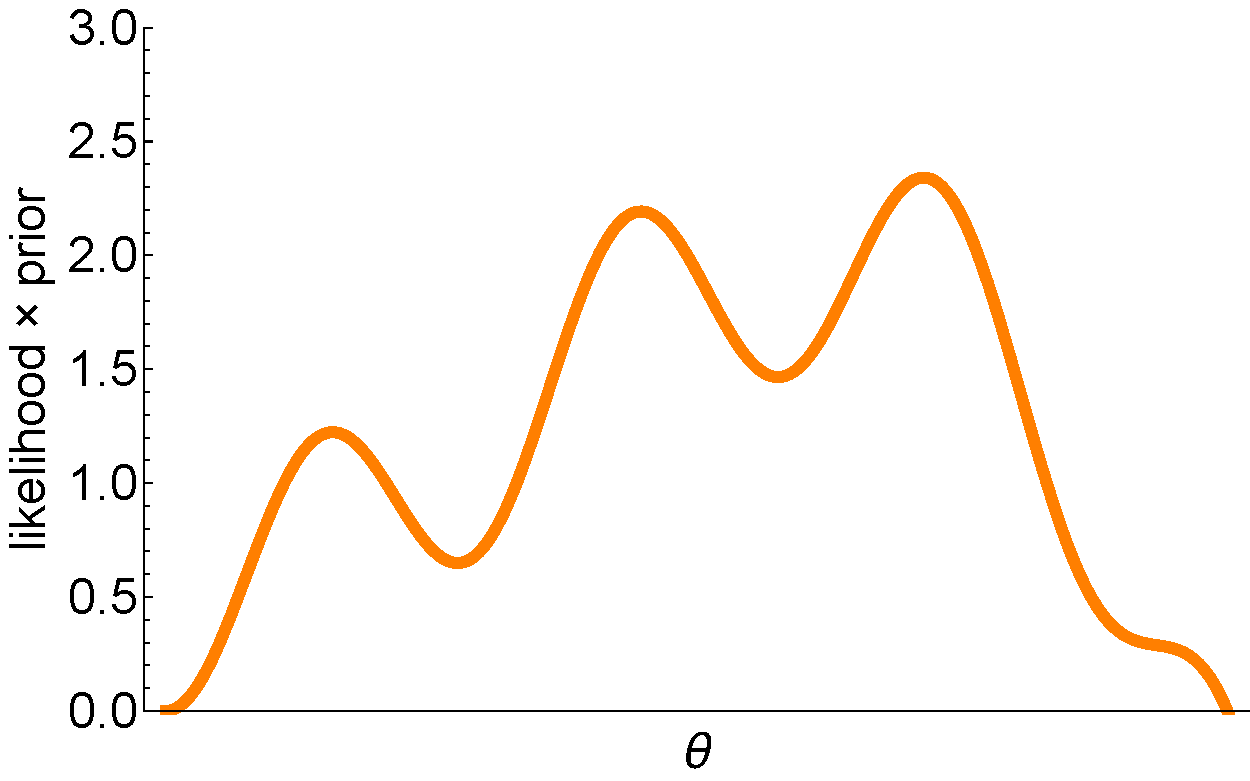
\includegraphics[width=1\textwidth]{./Figures/lec4_metropolisDefinition1.pdf}}
\end{figure}

\end{frame}

\begin{frame}
\frametitle{Defining Random Walk Metropolis}
Select a random starting location.

\begin{figure}[ht]
\centerline{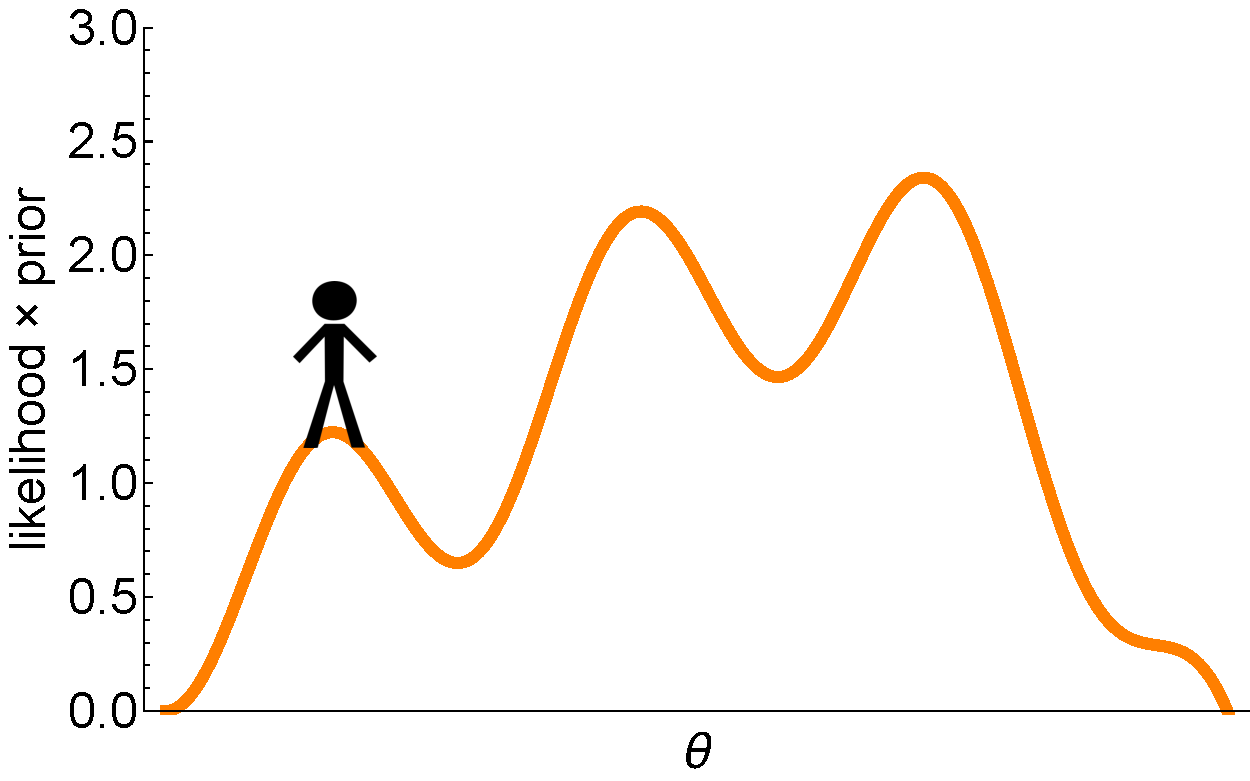
\includegraphics[width=1\textwidth]{./Figures/lec4_metropolisDefinition2.pdf}}
\end{figure}

\end{frame}

\begin{frame}
\frametitle{Defining Random Walk Metropolis}
Propose a new location using jumping distribution.

\begin{figure}[ht]
\centerline{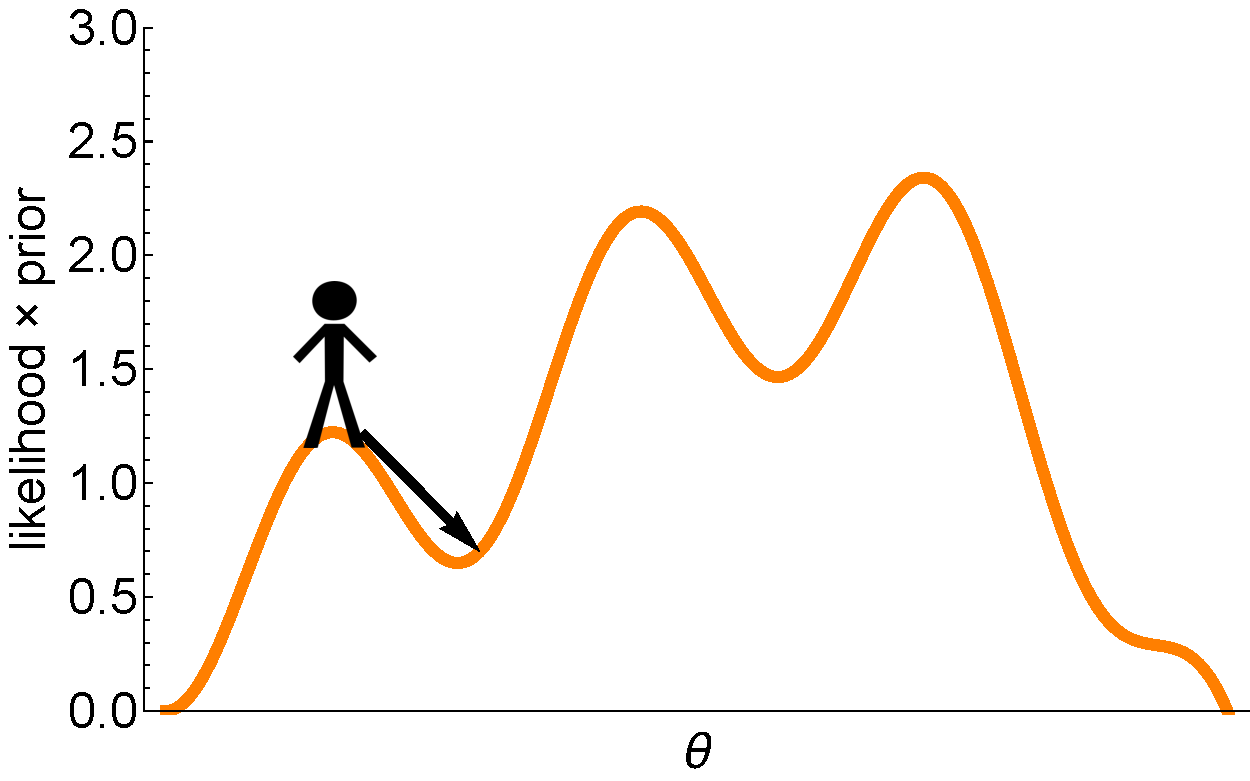
\includegraphics[width=1\textwidth]{./Figures/lec4_metropolisDefinition3.pdf}}
\end{figure}

\end{frame}

\begin{frame}
\frametitle{Defining Random Walk Metropolis}
Calculate ratio of likelihood $\times$ prior at proposed to current location, and find $r \approx 0.58$.

\begin{figure}[ht]
\centerline{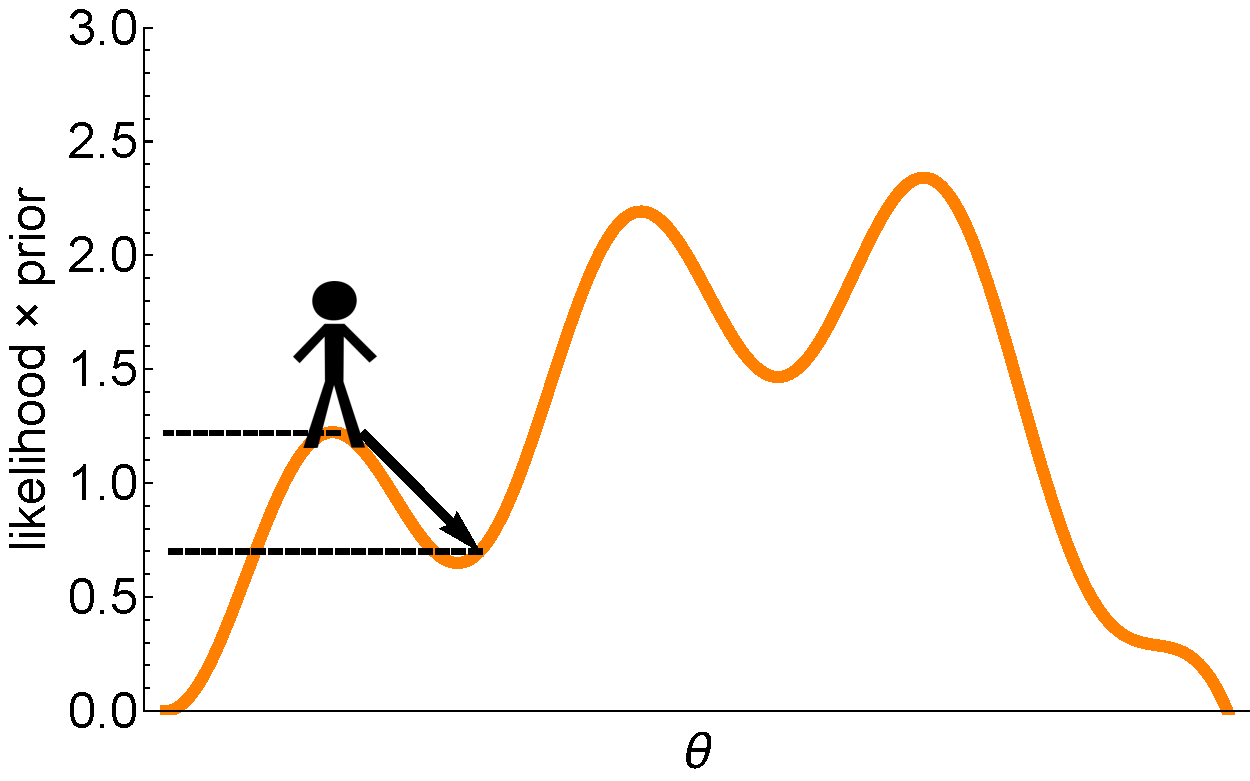
\includegraphics[width=1\textwidth]{./Figures/lec4_metropolisDefinition4.pdf}}
\end{figure}

\end{frame}

\begin{frame}
\frametitle{Defining Random Walk Metropolis}
Compare $r \approx 0.58$ with random real between 0 and 1. For example suppose we obtain $u = 0.823$.

\begin{figure}[ht]
\centerline{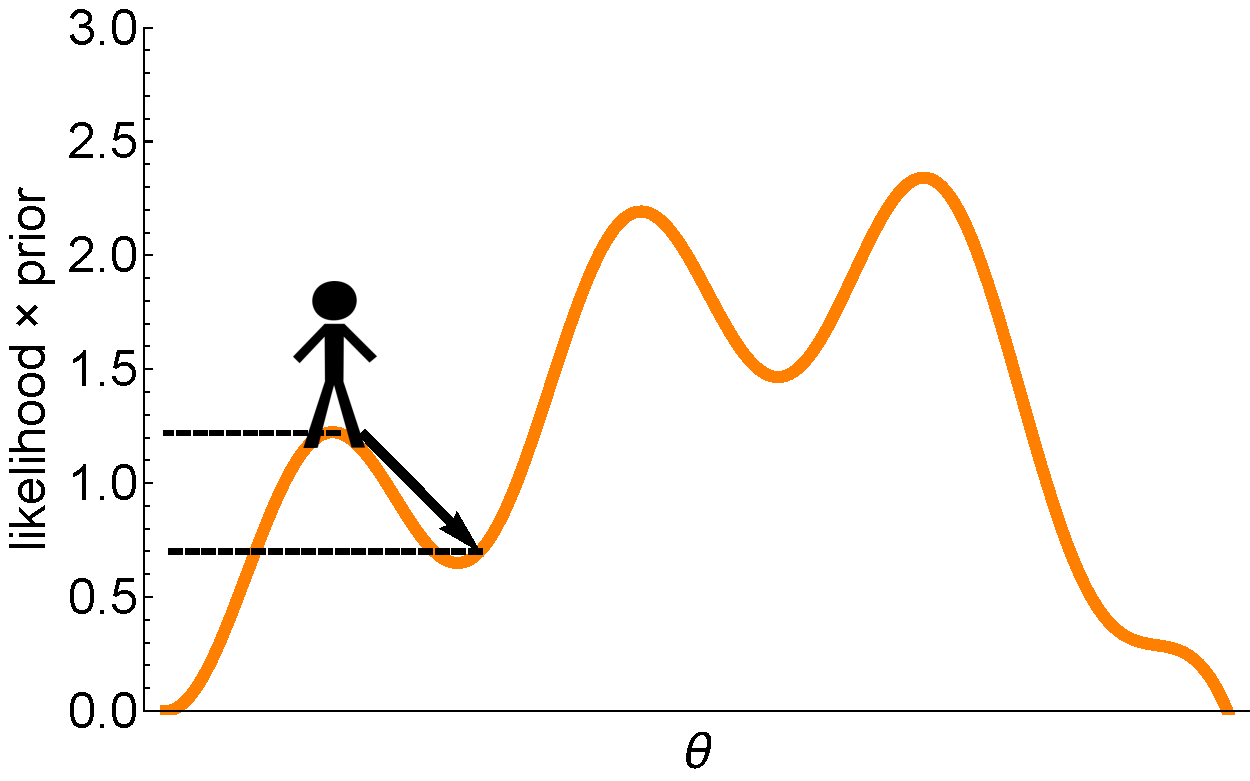
\includegraphics[width=1\textwidth]{./Figures/lec4_metropolisDefinition4.pdf}}
\end{figure}

\end{frame}

\begin{frame}
\frametitle{Defining Random Walk Metropolis}
Since $r < u$ we remain at our original location.

\begin{figure}[ht]
\centerline{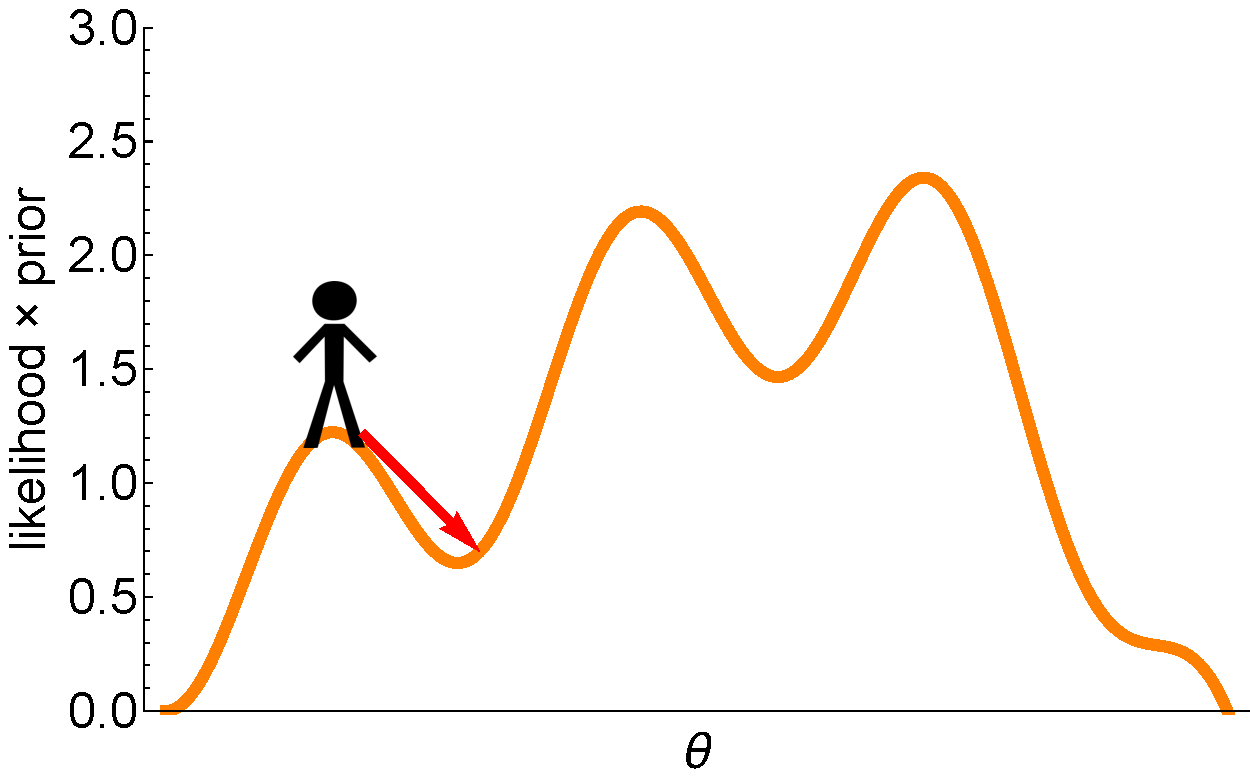
\includegraphics[width=1\textwidth]{./Figures/lec4_metropolisDefinition5.pdf}}
\end{figure}

\end{frame}

\begin{frame}
\frametitle{Defining Random Walk Metropolis}
Generate a new proposed step using jumping distribution.

\begin{figure}[ht]
\centerline{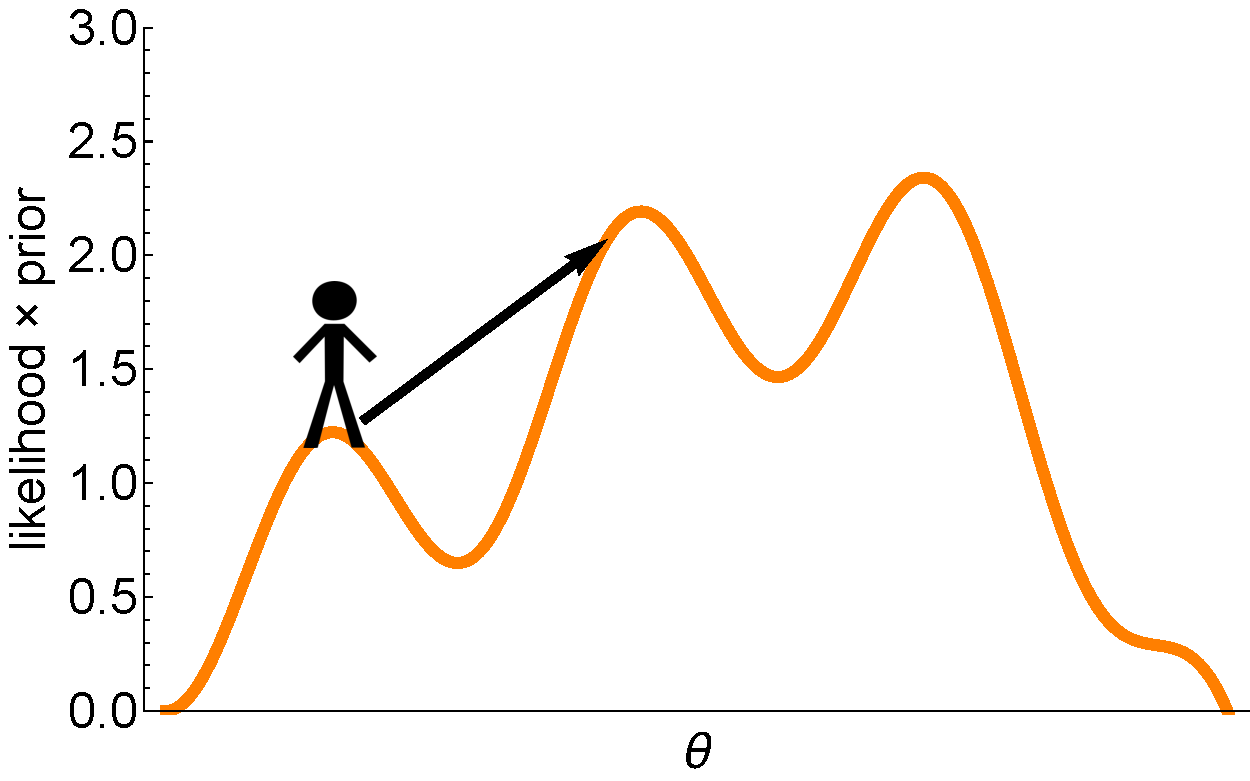
\includegraphics[width=1\textwidth]{./Figures/lec4_metropolisDefinition6.pdf}}
\end{figure}

\end{frame}

\begin{frame}
\frametitle{Defining Random Walk Metropolis}
Calculate ratio of likelihood $\times$ prior at proposed to current location, and find $r \approx 1.75$.

\begin{figure}[ht]
\centerline{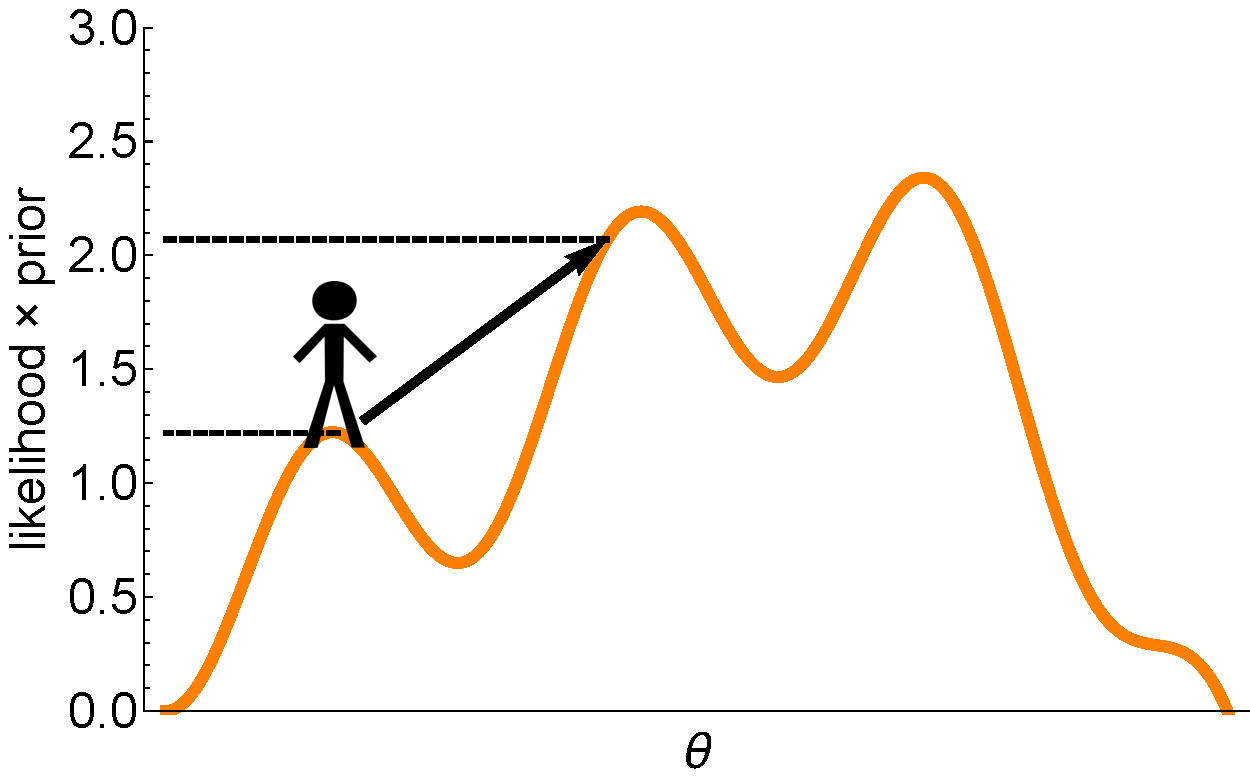
\includegraphics[width=1\textwidth]{./Figures/lec4_metropolisDefinition7.pdf}}
\end{figure}

\end{frame}

\begin{frame}
\frametitle{Defining Random Walk Metropolis}
Since $r > 1$ (maximum possible $u$) $\implies$ we move to new location.

\begin{figure}[ht]
\centerline{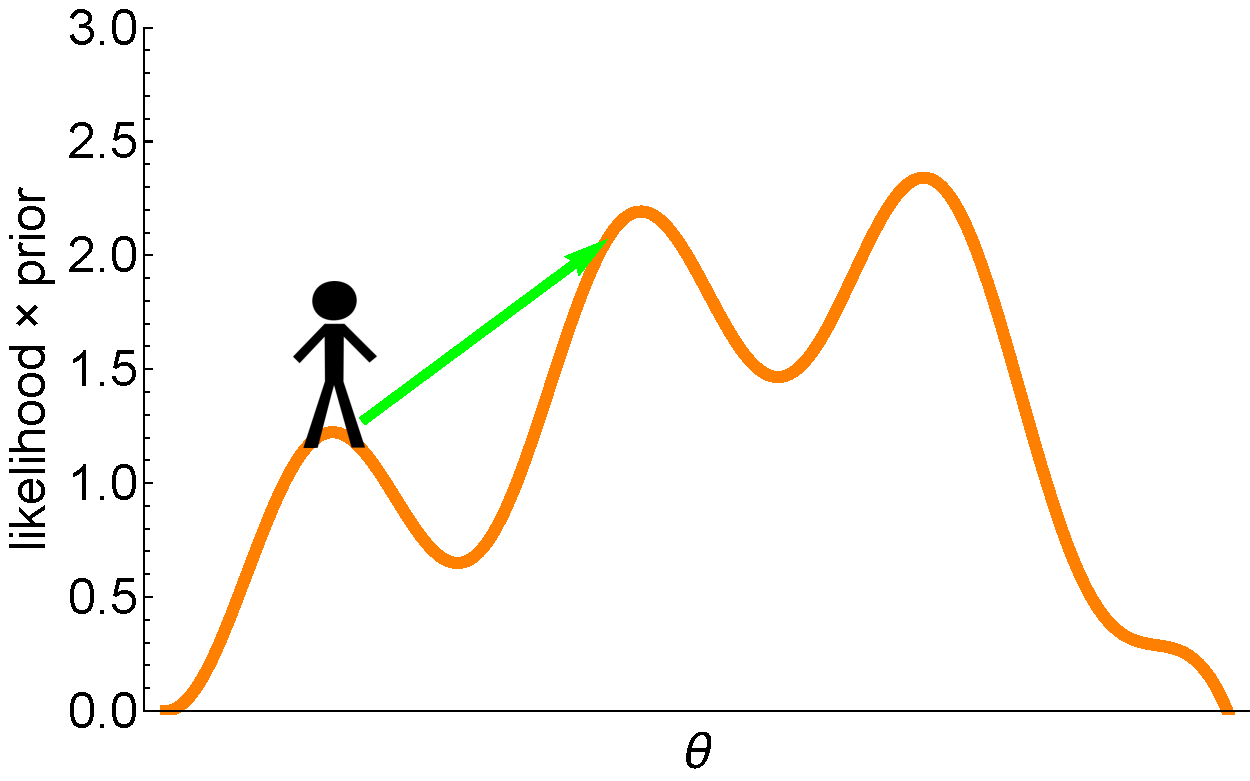
\includegraphics[width=1\textwidth]{./Figures/lec4_metropolisDefinition8.pdf}}
\end{figure}

\end{frame}

\begin{frame}
\frametitle{Defining Random Walk Metropolis}
Since $r > 1$ (maximum possible $u$) $\implies$ we move to new location.

\begin{figure}[ht]
\centerline{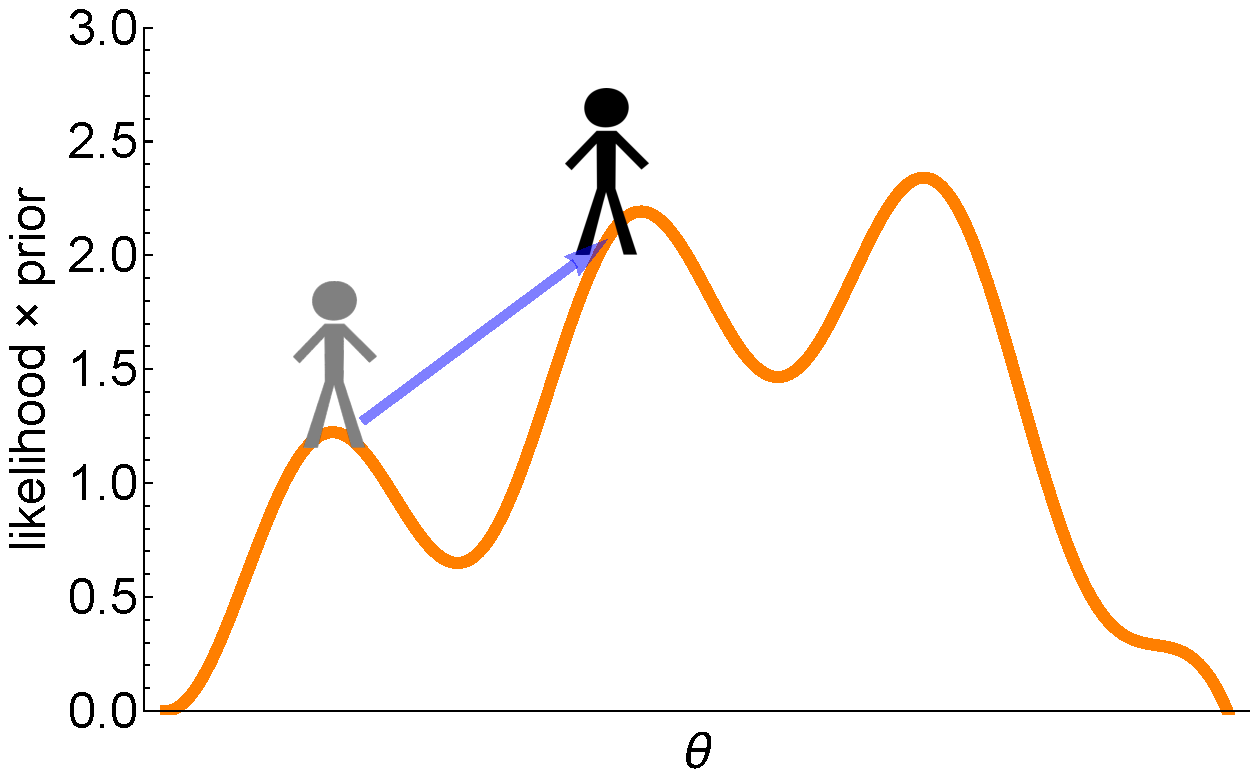
\includegraphics[width=1\textwidth]{./Figures/lec4_metropolisDefinition9.pdf}}
\end{figure}

\end{frame}

\begin{frame}
\frametitle{Defining Random Walk Metropolis}
Propose a new step using jumping distribution.

\begin{figure}[ht]
\centerline{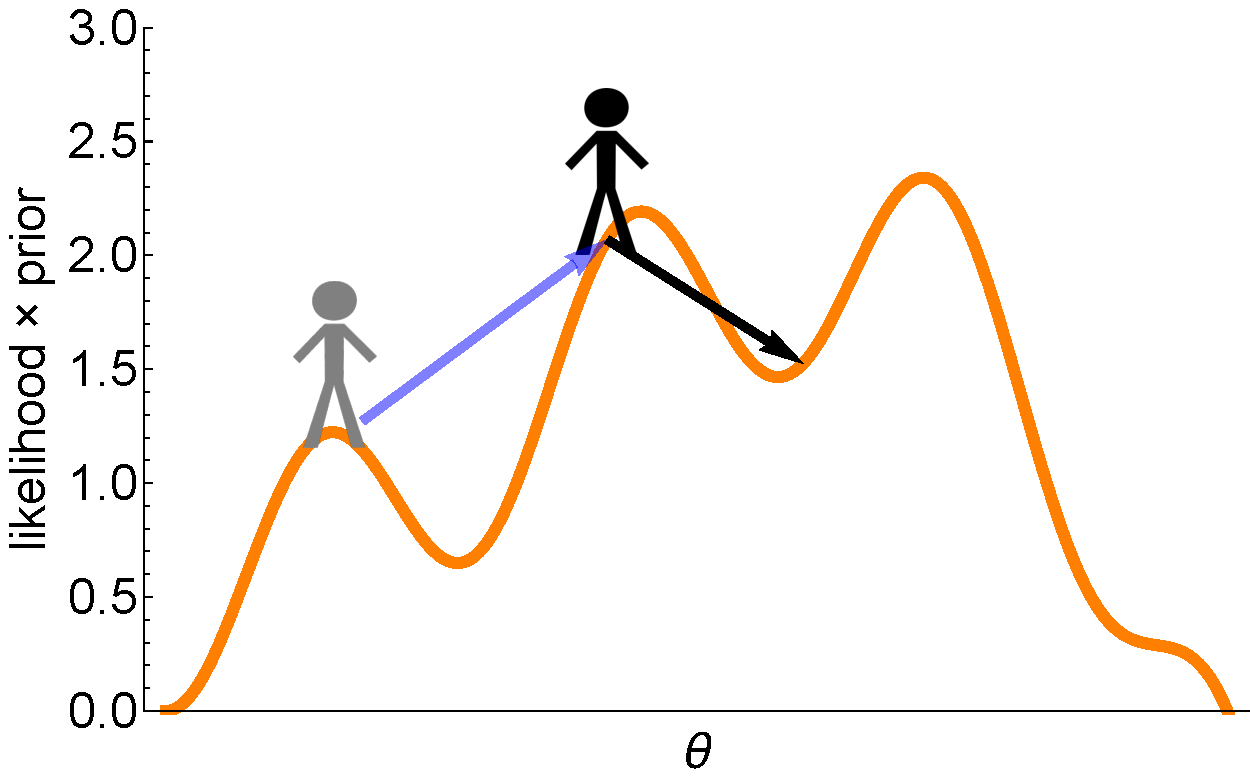
\includegraphics[width=1\textwidth]{./Figures/lec4_metropolisDefinition10.pdf}}
\end{figure}

\end{frame}

\begin{frame}
\frametitle{Defining Random Walk Metropolis}
Calculate $r\approx 0.75$.

\begin{figure}[ht]
\centerline{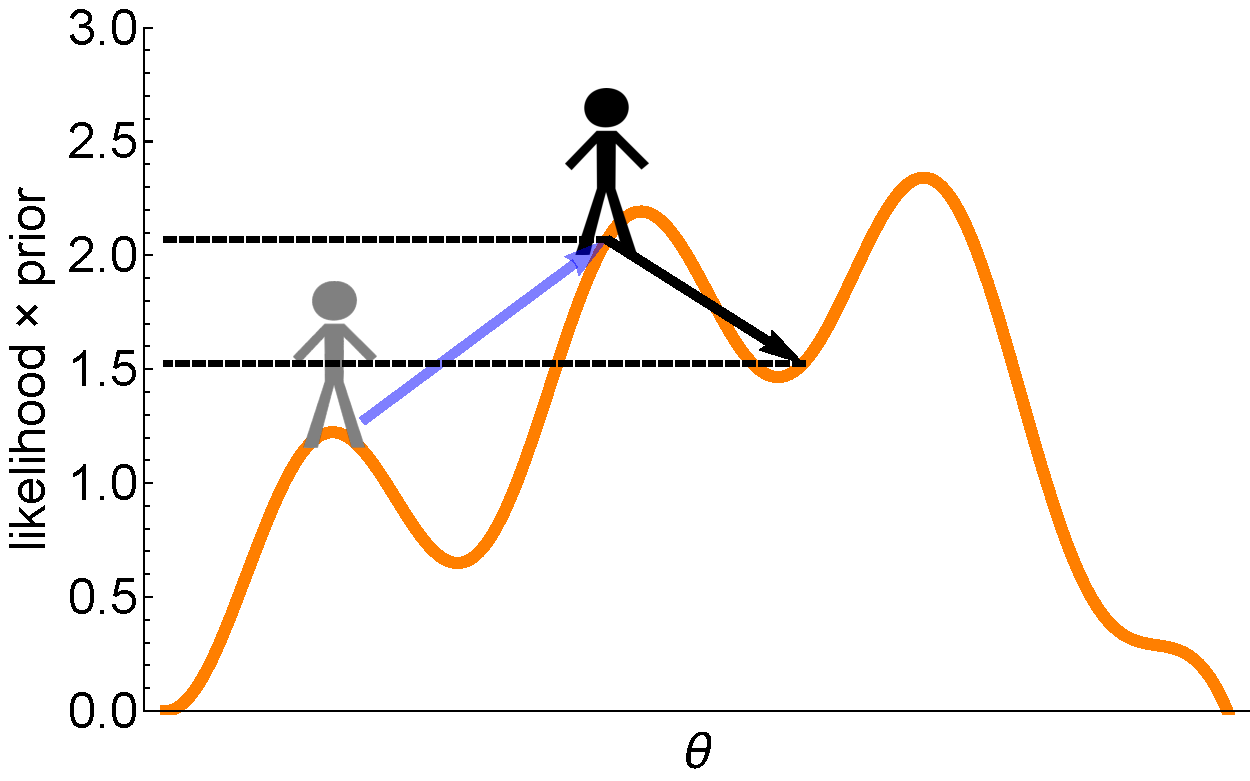
\includegraphics[width=1\textwidth]{./Figures/lec4_metropolisDefinition11.pdf}}
\end{figure}

\end{frame}

\begin{frame}
\frametitle{Defining Random Walk Metropolis}
Generate $u = 0.278 < r$ $\implies$ we move! 

\begin{figure}[ht]
\centerline{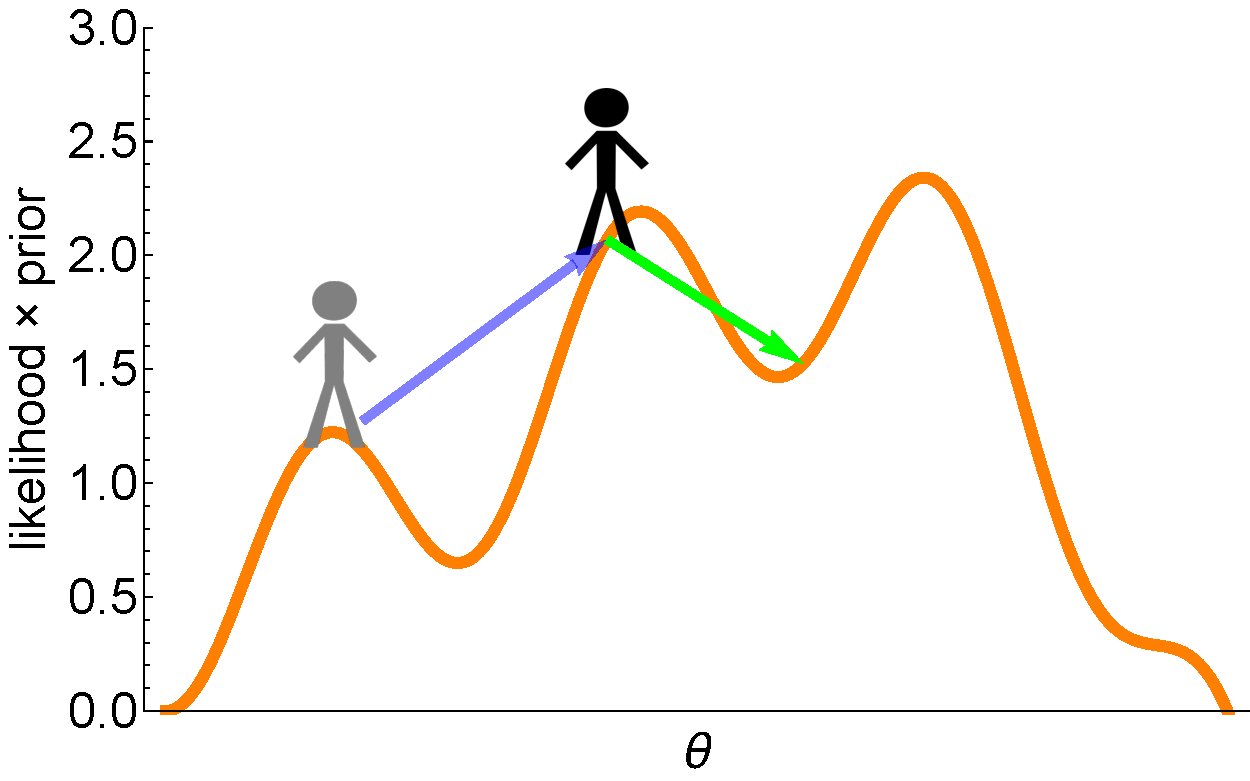
\includegraphics[width=1\textwidth]{./Figures/lec4_metropolisDefinition12.pdf}}
\end{figure}

\end{frame}

\begin{frame}
\frametitle{Defining Random Walk Metropolis}
Generate $u = 0.278 < r$ $\implies$ we move! 

\begin{figure}[ht]
\centerline{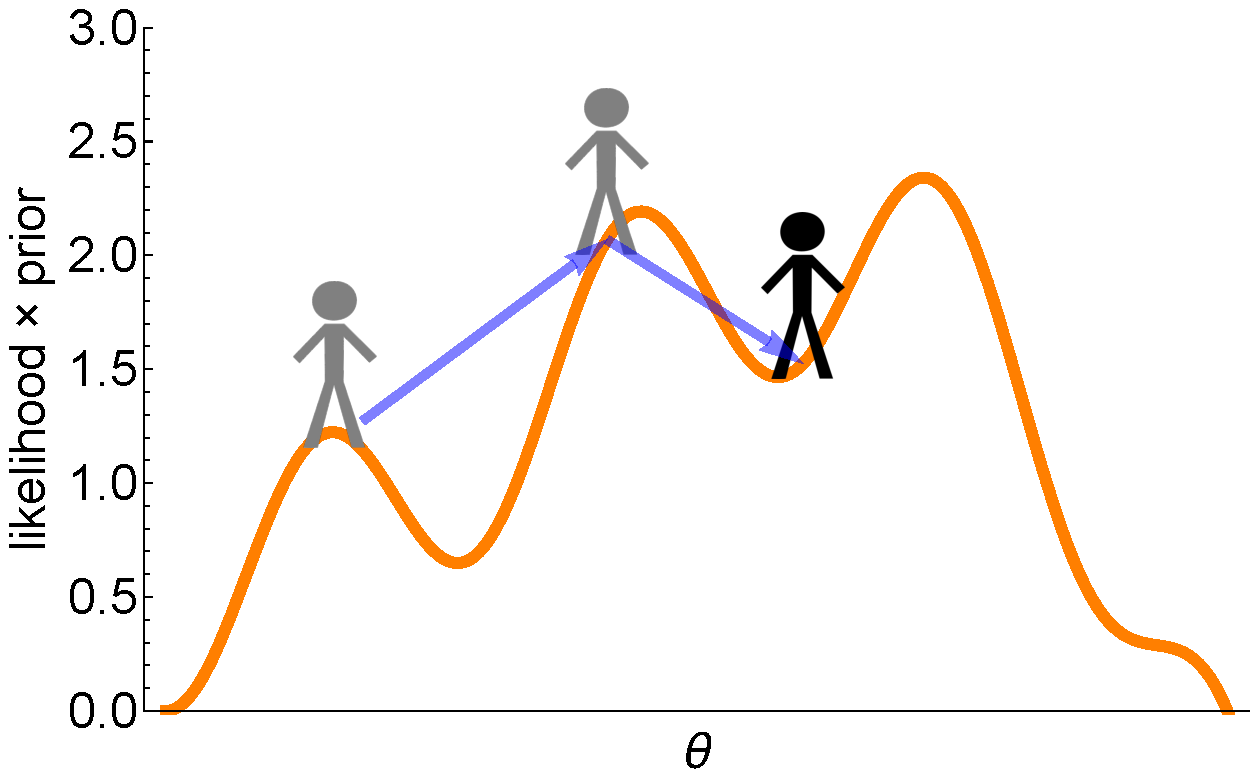
\includegraphics[width=1\textwidth]{./Figures/lec4_metropolisDefinition13.pdf}}
\end{figure}

\end{frame}

\begin{frame}
\frametitle{Defining Random Walk Metropolis}
Repeat a large number of times.

\begin{figure}[ht]
\centerline{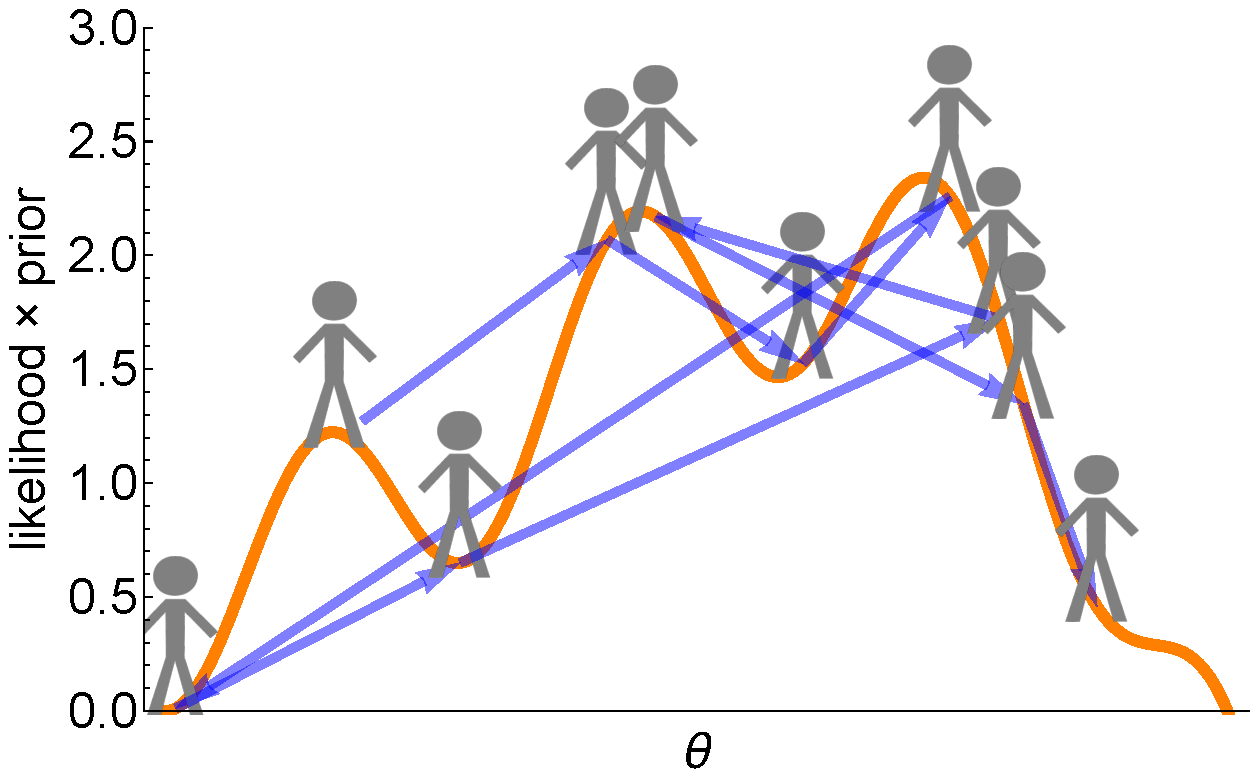
\includegraphics[width=1\textwidth]{./Figures/lec4_metropolisDefinitionFinal.pdf}}
\end{figure}

\end{frame}

\begin{frame}
\frametitle{Random Walk Metropolis: benefits}

\begin{itemize}
\item<2-> Under quite general conditions the Random Walk Metropolis sampler converges \textbf{asymptotically} to the posterior.
\item<3-> However for a sufficiently large sample size the sampling distribution may be practically indistinguishable from the true posterior.
\item<4-> The algorithm requires us to be able to calculate the ratio:
\onslide<5->
\begin{equation}
r = \frac{\text{likelihood}(\theta_{t+1})\times\text{prior}(\theta_{t+1})}{\text{likelihood}(\theta_{t})\times\text{prior}(\theta_{t})}
\end{equation}
\item<6-> The ratio uses \textbf{only} the numerator of Bayes' rule $\implies$ we side-step calculating the denominator!
\end{itemize}

\end{frame}

\begin{frame}
\frametitle{Random Walk Metropolis in action}
Can we use Random Walk Metropolis to sample from the continuous distribution below?
\visible<2->{
\begin{figure}[ht]
\centerline{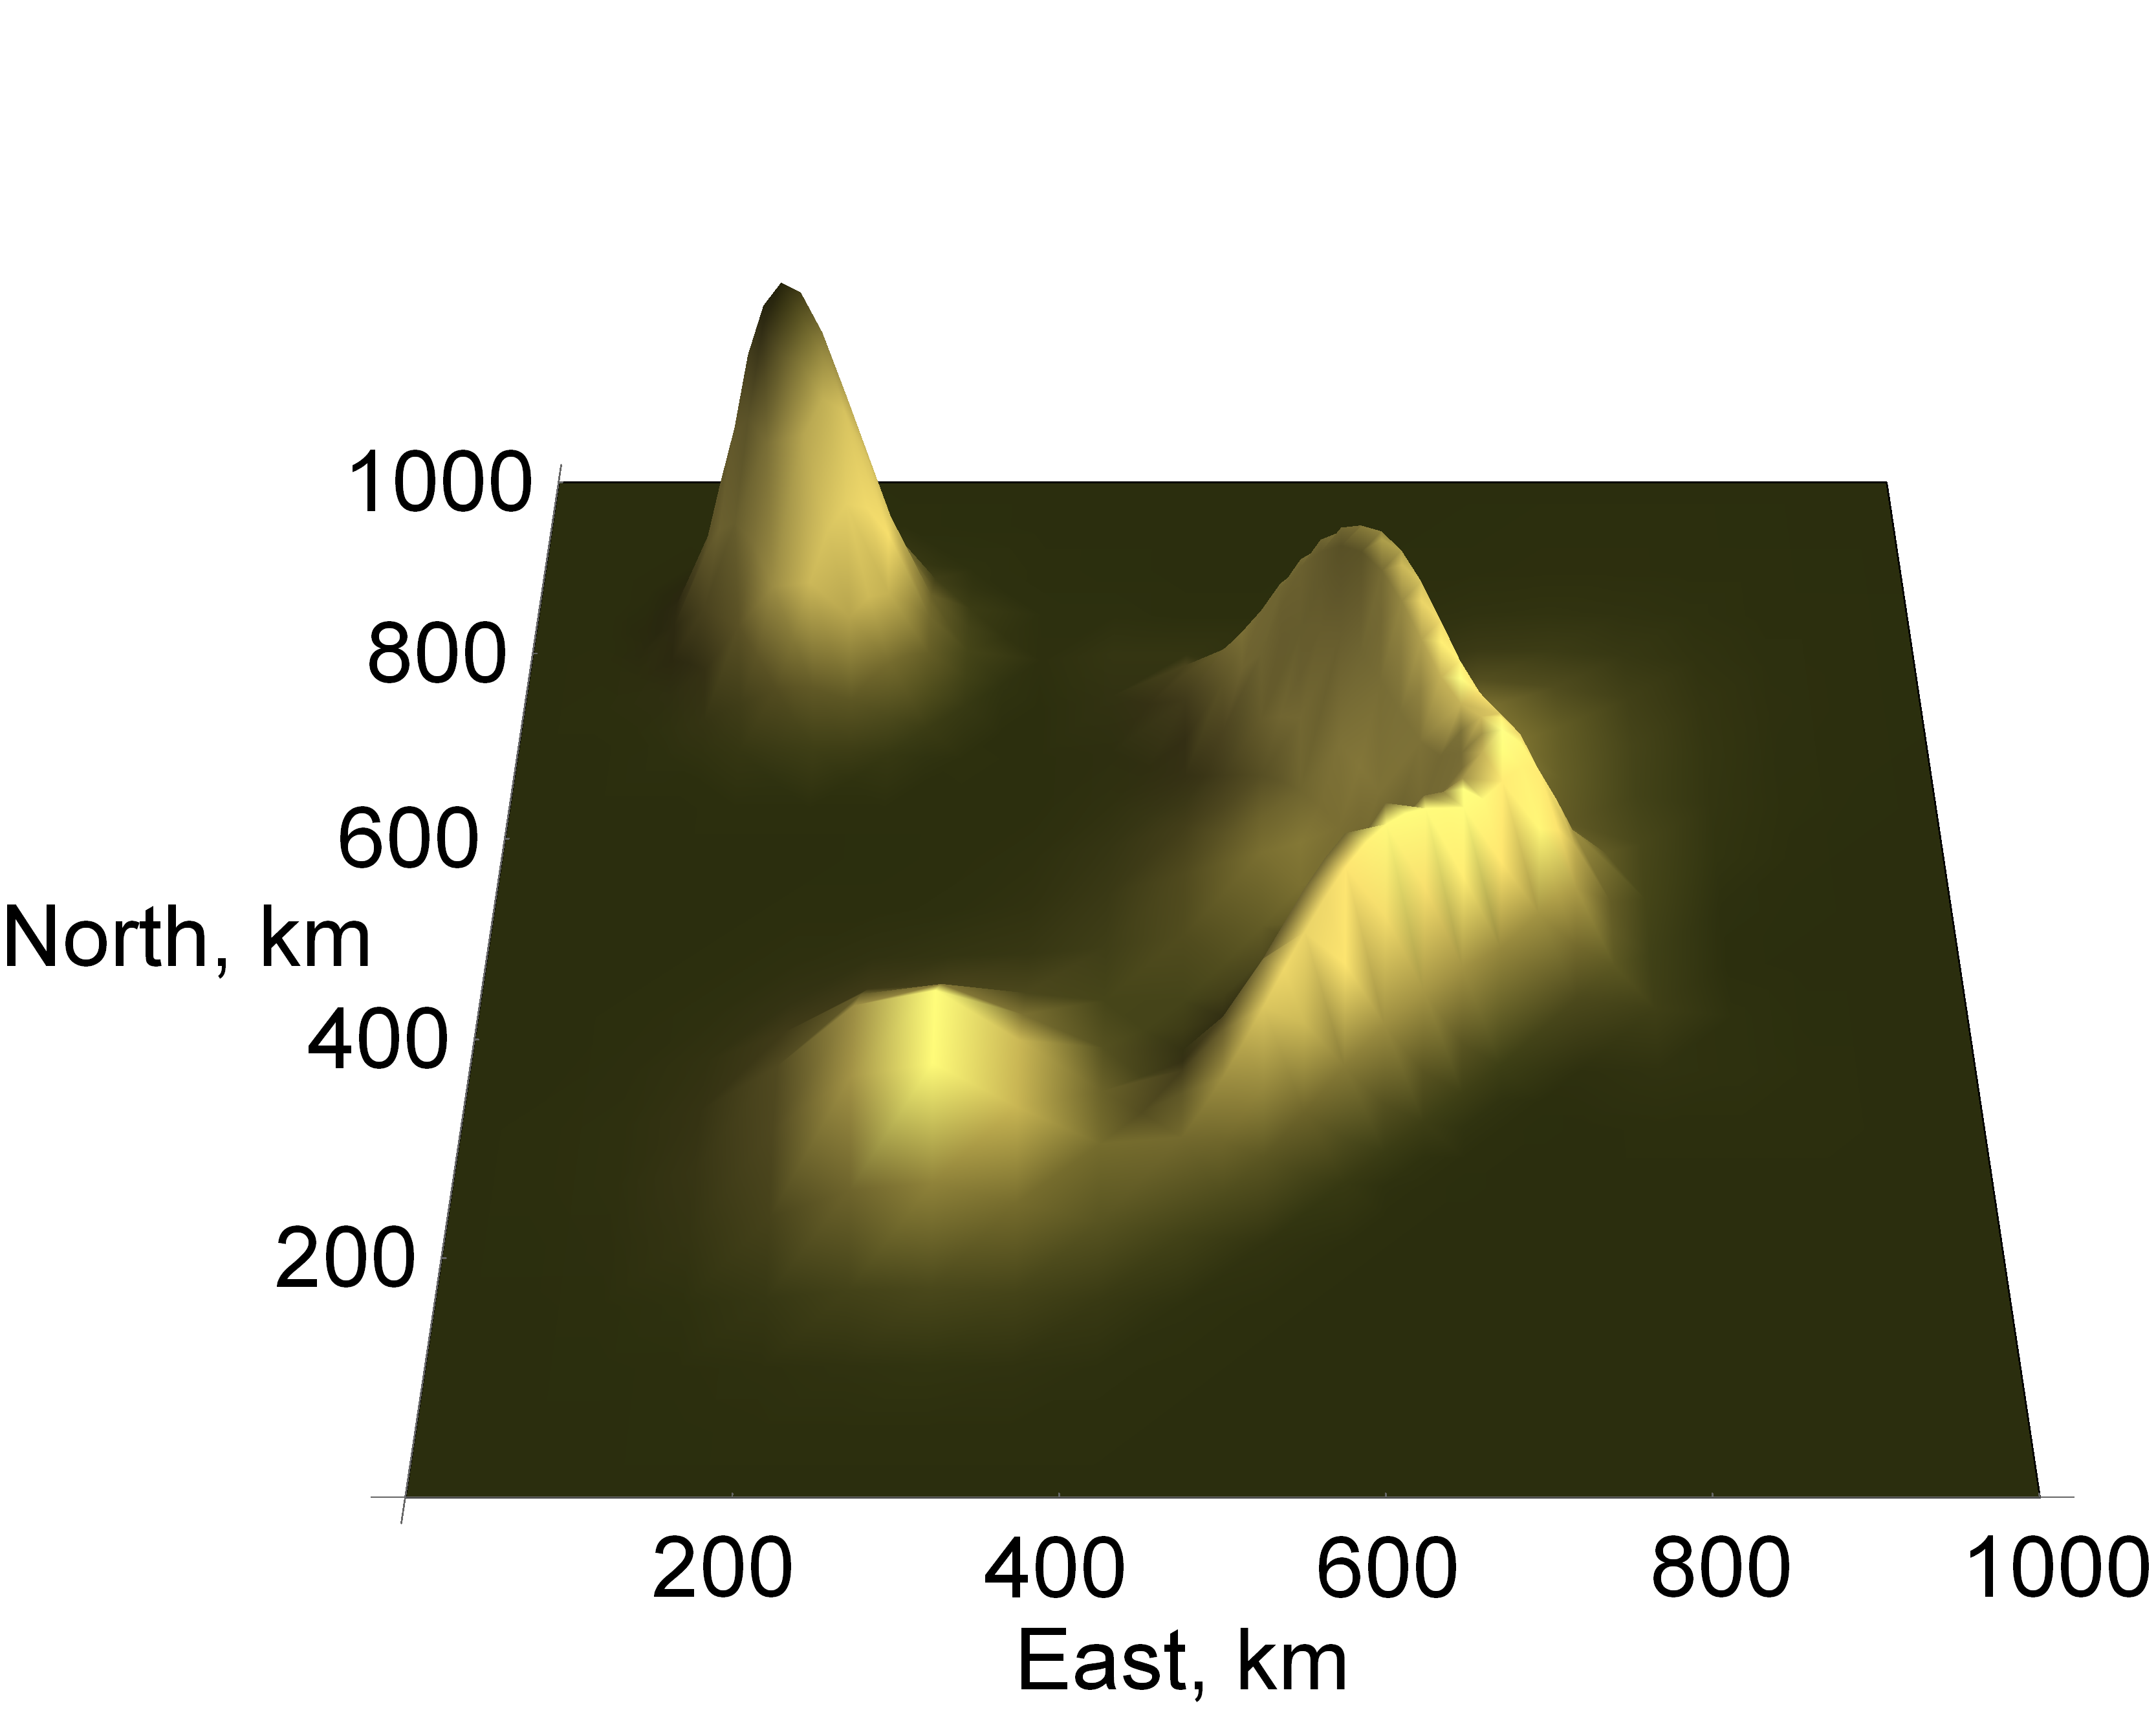
\includegraphics[width=0.8\textwidth]{./Figures/lec4_goldMiningActual.png}}
\end{figure}}
\end{frame}

\begin{frame}
\frametitle{Random Walk Metropolis in action}
\begin{figure}[t]
\centerline{\animategraphics[width=0.75\textwidth,controls,buttonsize=1em,buttonfg=0.5]{2}{./Figures/lec4_goldMineAccept}{1}{101}}
\end{figure}

\end{frame}

\begin{frame}
\frametitle{Random Walk Metropolis in action}

\begin{figure}[t]
\centerline{\animategraphics[width=1\textwidth,controls,buttonsize=1em,buttonfg=0.5]{2}{./Figures/lec4_goldMining3D}{1}{48}}
\end{figure}

\end{frame}

\begin{frame}
\frametitle{Random Walk Metropolis: short summary}

\begin{itemize}
\item<2-> Algorithm works by starting in a randomly-determined position in parameter space.
\item<3-> In each iteration we generate a proposed (local) step from our current position.
\item<4-> We then move based the ratio of the proposed \textbf{un-normalised} posterior to our current location $\implies$ no need to calculate troublesome denominator.
\item<5-> The path of our positions over time forms our \textbf{sample}.
\item<6-> If we repeat the above for a (large) number of steps $\implies$ sampling distribution $\approx$ posterior.
\end{itemize}

\end{frame}

\begin{frame}
\frametitle{How do we choose the jumping distribution?}

\begin{itemize}
\item<2-> Sometimes called the ``proposal distribution''.
\item<3-> In Random Walk Metropolis we use a symmetric distribution (relaxed in Metropolis-Hastings):
\onslide<4-> $\implies J(\theta_a|\theta_b) = J(\theta_b|\theta_a)$
\end{itemize}

\visible<5->{
\begin{figure}[ht]
\centerline{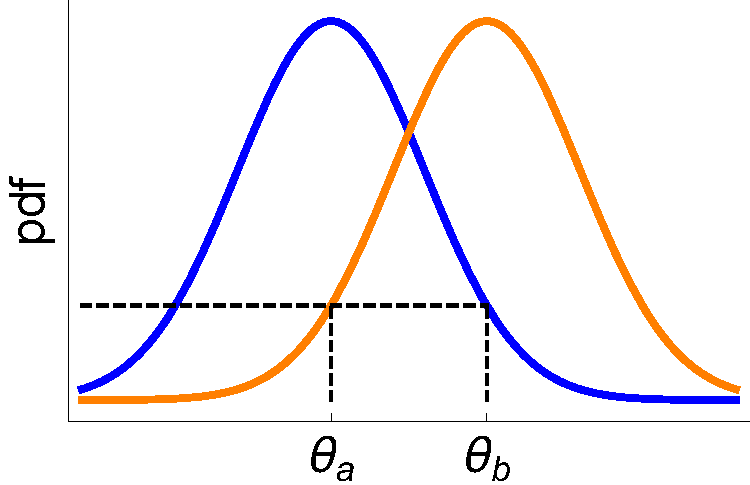
\includegraphics[width=0.8\textwidth]{./Figures/lec4_normalProposal.pdf}}
\end{figure}}

\end{frame}

\begin{frame}
\frametitle{The importance of step size}
\textbf{Question:} how should we decide on the jumping kernel's step size?

\visible<1->{
\begin{figure}[ht]
\centerline{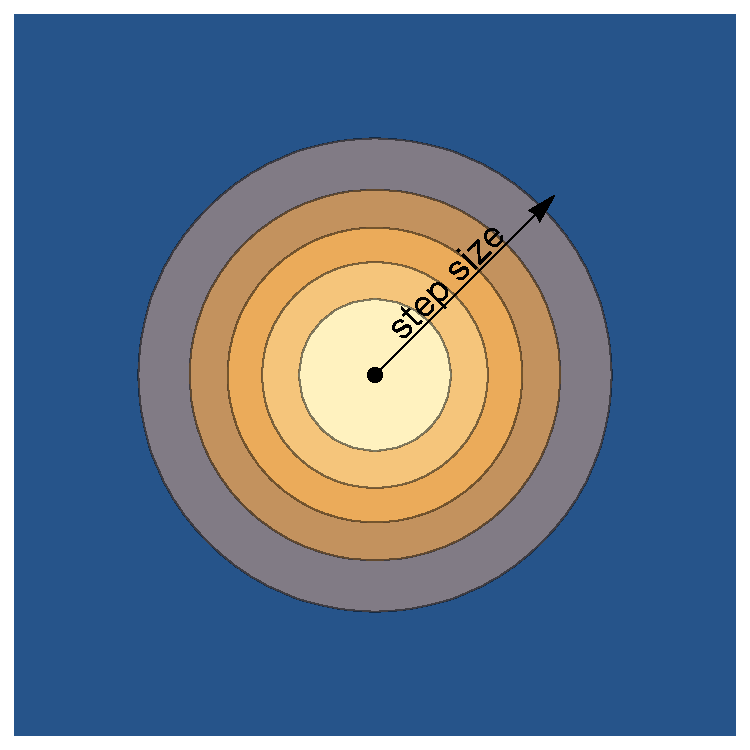
\includegraphics[width=0.6\textwidth]{./Figures/lec4_stepSizeKernel.pdf}}
\end{figure}}

\end{frame}

\begin{frame}
\frametitle{Another example posterior distribution}
Assume a unimodal distribution from which we want to sample.

\begin{figure}[ht]
\centerline{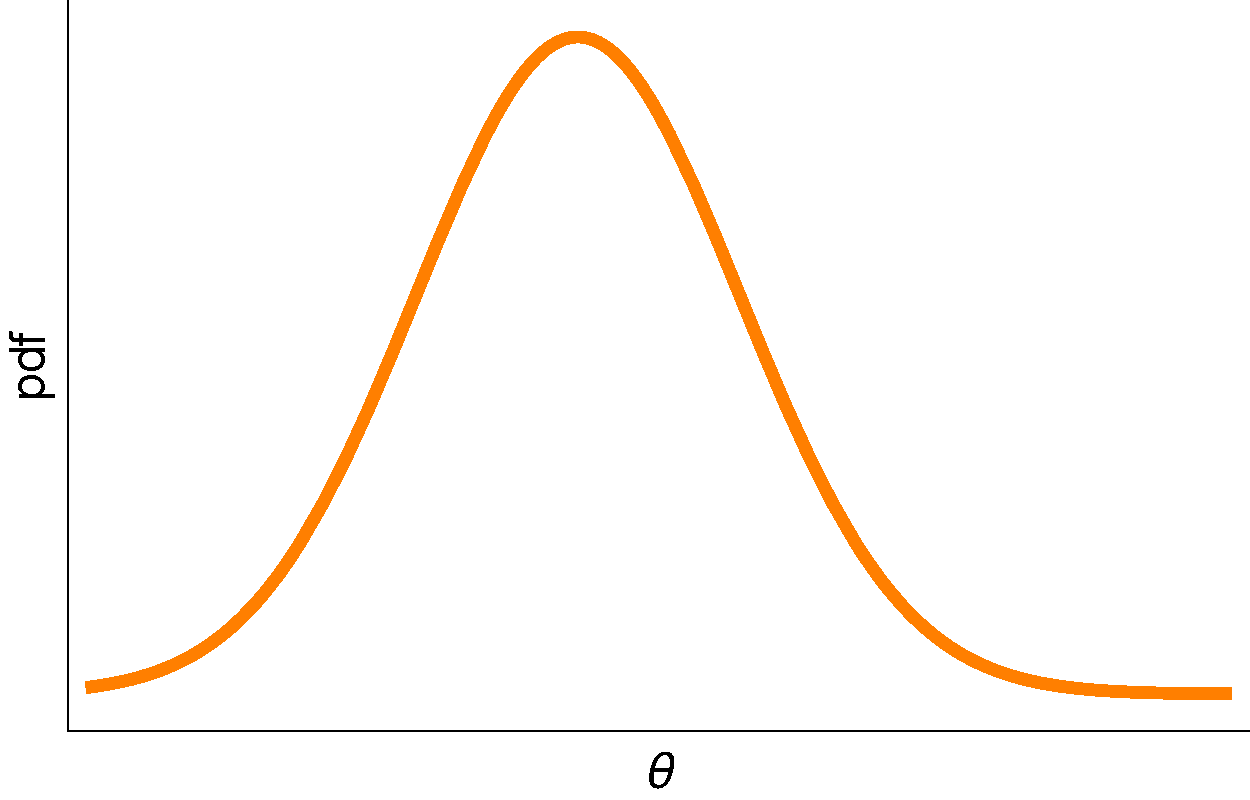
\includegraphics[width=0.8\textwidth]{./Figures/lec4_stepSizeStart1.pdf}}
\end{figure}

\end{frame}

\begin{frame}
\frametitle{Another example posterior distribution}
Start three algorithms with different step sizes at same point.

\begin{figure}[ht]
\centerline{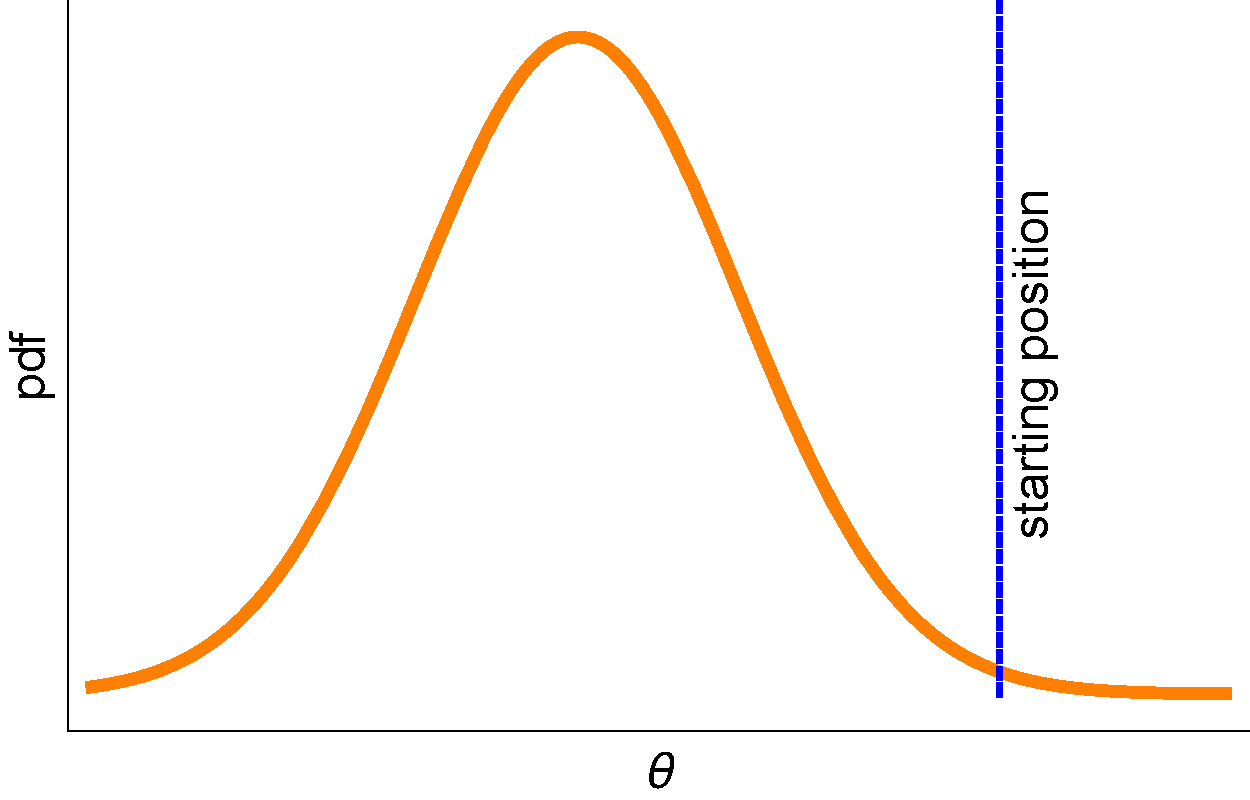
\includegraphics[width=0.8\textwidth]{./Figures/lec4_stepSizeStart2.pdf}}
\end{figure}

\end{frame}

\begin{frame}
\frametitle{The importance of step size: too small}

\begin{figure}[t]
\centerline{\animategraphics[width=0.85\textwidth,controls,buttonsize=1em,buttonfg=0.5]{2}{./Figures/lec4_step_small}{1}{20}}
\end{figure}

\end{frame}

\begin{frame}
\frametitle{The importance of step size: too large}

\begin{figure}[t]
\centerline{\animategraphics[width=0.85\textwidth,controls,buttonsize=1em,buttonfg=0.5]{2}{./Figures/lec4_step_large}{1}{20}}
\end{figure}

\end{frame}

\begin{frame}
\frametitle{The importance of step size: just right}

\begin{figure}[t]
\centerline{\animategraphics[width=0.85\textwidth,controls,buttonsize=1em,buttonfg=0.5]{2}{./Figures/lec4_step_correct}{1}{20}}
\end{figure}

\end{frame}

\begin{frame}
\frametitle{Step size: summary}
\begin{itemize}
\item<2-> Whilst step size does not affect asymptotic convergence, it does affect finite sample performance.
\item<3-> If step size is too small we do not find the typical set (area of high probability mass). 
\item<4-> If step size is too large we find the typical set, but do not explore it efficiently.
\item<5-> Therefore do an initial run of sampler to find optimal step size before starting proper.
\end{itemize}

\end{frame}

\section{Judging convergence of chains to posterior}
\frame{\tableofcontents[currentsection]}


\begin{frame}
\frametitle{Why do we need to monitor convergence?}
Recap the steps of Metropolis:
\begin{enumerate}
\item<2-> Propose an initial position $\theta_0$ using a initial proposal distribution $\pi(\theta)\neq p(\theta|X)$.
\item<3-> For $t=1,...,T$ do:
\begin{itemize}
\item<4-> Propose a new location:
 $\theta_{t+1}\sim J(\theta_{t+1}|\theta_t)$.
\item<5-> Accept/reject move based on
\begin{equation}
r = \frac{p(X|\theta_{t+1}) p(\theta_{t+1})}{p(X|\theta_{t}) p(\theta_{t})} > u\sim Unif(0,1)
\end{equation}
\end{itemize}
\end{enumerate}

\end{frame}


\begin{frame}
\frametitle{Why do we need to monitor convergence?}
\begin{itemize}
\item<2-> Start with an initial proposal distribution $\pi(\theta)\neq p(\theta|X)$.
\item<3-> Repeatedly take steps and use the Metropolis accept/reject rule $\implies$ $\pi(\theta_t)$; the sampling distribution at time $t$.
\item<4-> Under a set of quite general assumptions we are guaranteed that asymptotically: $\pi(\theta_t)\rightarrow p(\theta|X)$.
\item<5-> However, when practically can we assume: $\pi(\theta_t)\approx p(\theta|X)$?
\end{itemize}
\end{frame}

\begin{frame}
\frametitle{How to measure convergence?}
\begin{itemize}
\item<2-> To monitor convergence to the posterior $\implies$ need the posterior.
\item<3-> But we don't have the posterior $\impliedby$ the reason we are doing the sampling in the first place!
\end{itemize}

\begin{figure}[ht]
\centerline{
\includegraphics[width=0.8\textwidth]{./Figures/catch-22-quote.jpg}}
\end{figure}

\end{frame}

\begin{frame}
\frametitle{Two strategies for monitoring convergence}

\onslide<2->\textbf{Strategy 1:} measure distributional separation.
\begin{itemize}
\item<3-> For example Kullback-Leibler:

\onslide<4->
\begin{equation}
KL=\int p(\theta|X) log\left(\frac{p(\theta|X)}{\pi(\theta_t)}\right) \mathrm{d}\theta
\end{equation}

\item<5-> Motivated by information theory.
\item<6-> Can use un-normalised posterior to do this.
\item<7-> Again integral is too difficult to do.
\end{itemize}

\onslide<1->
\begin{figure}[ht]
\centerline{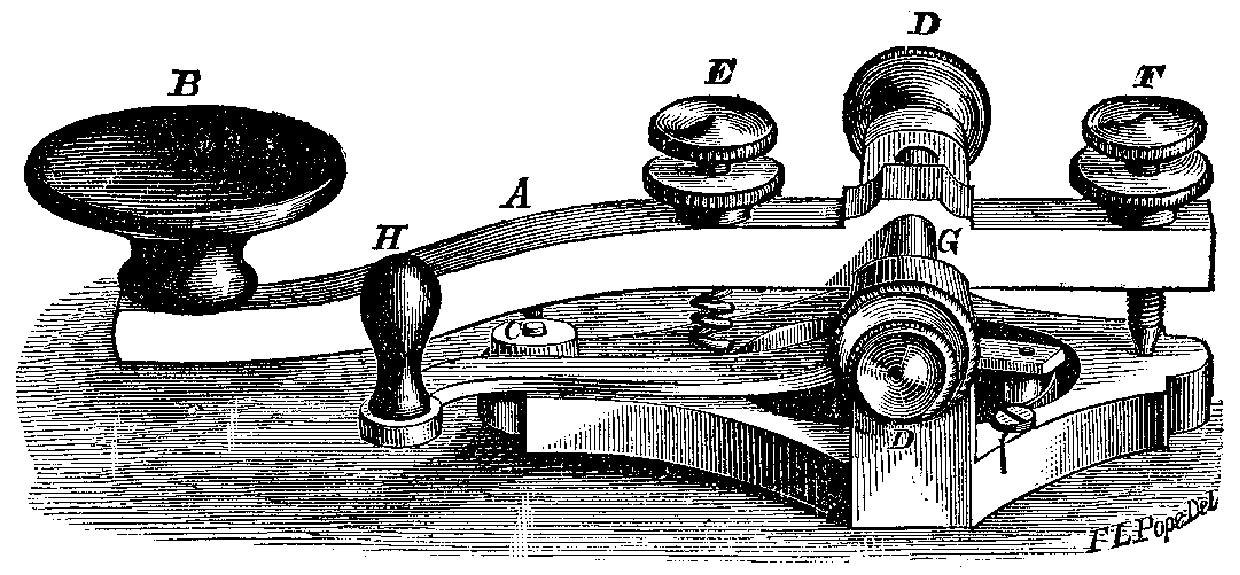
\includegraphics[width=1\textwidth]{./Figures/morse.pdf}}
\end{figure}

\end{frame}

\begin{frame}
\frametitle{Two strategies for monitoring convergence}

\onslide<2->\textbf{Strategy 2:} monitor the approach to a stationary distribution.

\begin{itemize}
\item<3-> We know asymptotically this will happen.
\item<4-> By design of Metropolis stepping and accept/reject rules, we know the stationary distribution is the posterior.
\end{itemize}

\onslide<1->
\begin{figure}[ht]
\centerline{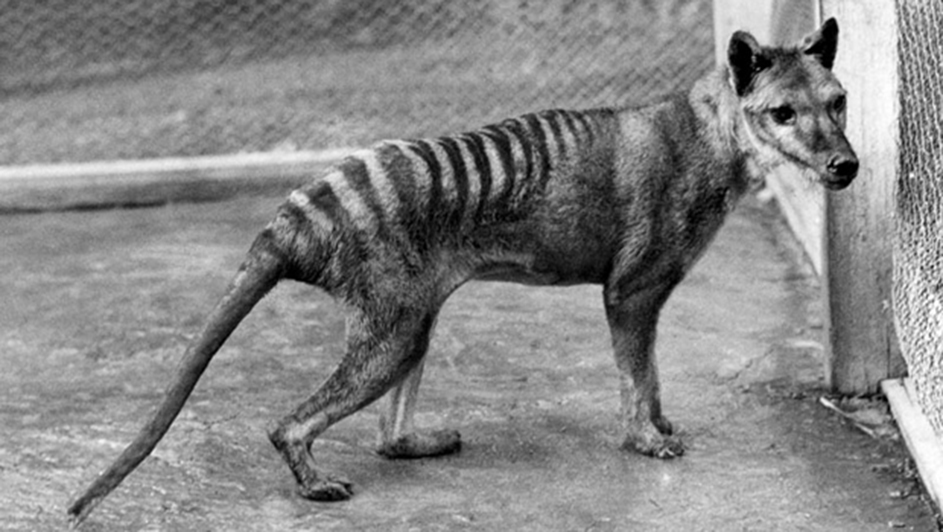
\includegraphics[width=1\textwidth]{./Figures/thylacine.jpg}}
\end{figure}

\end{frame}

\begin{frame}
\frametitle{Monitoring convergence of a single chain}

Initial idea:
\begin{itemize}
\item<2-> Compare summaries (mean, variance, etc.) of sampling distribution for a chain at time $t$ with itself at time $t+T$.
\item<3-> If their rate of change is below a threshold $\implies$ convergence.
\end{itemize}

\end{frame}

\begin{frame}
\frametitle{Monitoring convergence of a single chain}
\Large \textbf{Question:} What is the problem with this idea?
\end{frame}

\begin{frame}
\frametitle{Convergence monitoring: Bob's bees}
\onslide<2-> Thought experiment: 
\begin{itemize}
\item<2-> Imagine a house of unknown shape. 
\item<3-> We have an unlimited supply of bees, each equipped with a GPS tracker allowing us to accurately monitor their position.
\item<4-> \textbf{Question:} How can we use these to estimate the shape of the house?
\end{itemize}

\onslide<1->{
\begin{figure}[ht]
\centerline{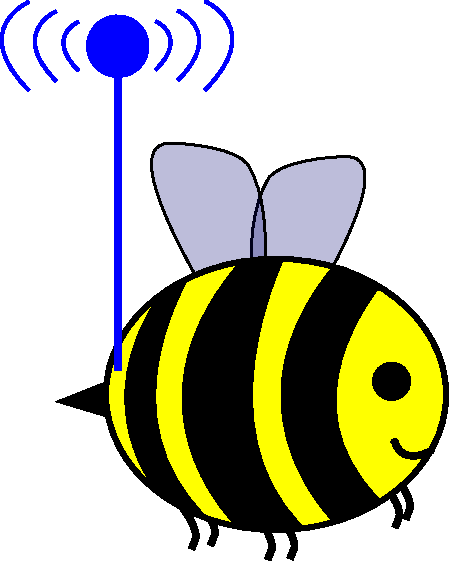
\includegraphics[width=0.3\textwidth]{./Figures/lec4_beeAntenna.pdf}}
\end{figure}}

\end{frame}

\begin{frame}
\frametitle{Convergence monitoring: Bob's bees}
\textbf{Answer}: 
\begin{itemize}
\item<2-> Release one (at a random location in the house) and monitor its path over time. 
\item<3-> Stop/collect bee after summary measures of its path stop changing.
\end{itemize}

\end{frame}

\begin{frame}
\frametitle{Convergence monitoring: single bee}

\begin{figure}[t]
\centerline{\animategraphics[width=1\textwidth,controls,buttonsize=1em,buttonfg=0.5]{8}{./Figures/lec4_beeSingleChaina}{1}{101}}
\end{figure}

\end{frame}

\begin{frame}
\frametitle{Convergence monitoring: single bee, a bit later}

\begin{figure}[t]
\centerline{\animategraphics[width=1\textwidth,controls,buttonsize=1em,buttonfg=0.5]{8}{./Figures/lec4_beeSingleChainb}{1}{101}}
\end{figure}

\end{frame}

\begin{frame}
\frametitle{Convergence monitoring: single bee, a bit bit later}

\begin{figure}[t]
\centerline{\animategraphics[width=1\textwidth,controls,buttonsize=1em,buttonfg=0.5]{8}{./Figures/lec4_beeSingleChainc}{1}{111}}
\end{figure}

\end{frame}

\begin{frame}
\frametitle{Convergence monitoring: single bee}
\Large \textbf{Question:} what's the actual shape of the house?

\end{frame}


\begin{frame}
\frametitle{Convergence monitoring: single bee}

\begin{figure}[t]
\centerline{\animategraphics[width=0.8\textwidth,controls,buttonsize=1em,buttonfg=0.5]{8}{./Figures/lec4_beeSingleChainBuilding}{1}{111}}
\end{figure}

\end{frame}

\begin{frame}
\frametitle{Single chain problems: summary}

\begin{itemize}
\item<2-> One way to monitor convergence is to look for convergence in a single chain's summary statistics.
\item<3-> This method is very susceptible to the curse of hindsight problem (``Now we've definitely converged on the posterior. We hadn't a minute ago.'')
\item<4-> Particularly because chains often get stuck in subregions of $\theta$ space. 
\end{itemize}

\end{frame}

\begin{frame}
\frametitle{The solutions: lots of bees}

\begin{itemize}
\item<2-> Release lots of bees starting at dispersed locations in parameter space.
\item<3-> Stop recording when an individual bee's path is indistinguishable from all others'.
\end{itemize}

\onslide<1->
\begin{figure}[ht]
\centerline{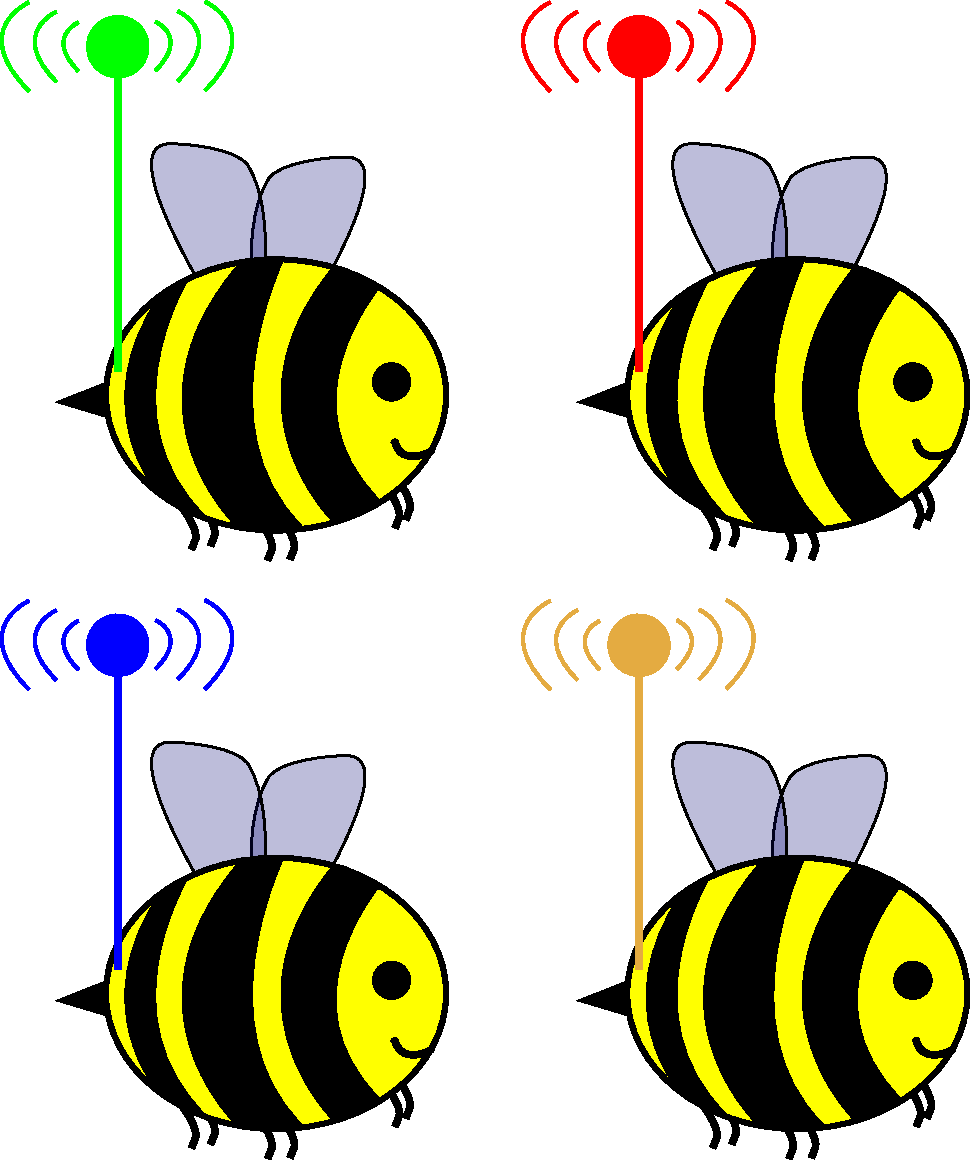
\includegraphics[width=0.3\textwidth]{./Figures/lec4_bees.pdf}}
\end{figure}

\end{frame}

\begin{frame}
\frametitle{Convergence monitoring: multiple bees}

\begin{figure}[t]
\centerline{\animategraphics[width=0.8\textwidth,controls,buttonsize=1em,buttonfg=0.5]{8}{./Figures/Lec4_beeMultipleChainWithouta}{1}{81}}
\end{figure}

\end{frame}

\begin{frame}
\frametitle{Convergence monitoring: multiple bees (a lot later)}

\begin{figure}[t]
\centerline{\animategraphics[width=0.8\textwidth,controls,buttonsize=1em,buttonfg=0.5]{8}{./Figures/lec4_beeMultipleChainWithoutFina}{1}{41}}
\end{figure}

\end{frame}

\begin{frame}
\frametitle{Multiple chain convergence monitoring: summary}

\begin{itemize}
\item<2-> Start a number of chains in random dispersed locations in $\theta$ space. 
\item<3-> Chains do \textit{not} interact with one another (in Metropolis).
\item<4-> Run each sampler until it is hard to distinguish one chain's path from all others'.
\item<5-> Less susceptible to ``curse of hindsight'', since we can see if chains aren't mixing.
\item<6-> Not foolproof! There still may be an area of high probability mass that we miss. However, less likely to fail compared to a single chain.
\item<7-> The more chains, the better!
\end{itemize}

\end{frame}

\begin{frame}
	\frametitle{Judging convergence}
	Single bee in a house.
	
	\begin{figure}[t]
		\centerline{\animategraphics[width=1\textwidth,controls,buttonsize=1em,buttonfg=0.5]{6}{./Figures/lec5_beeSingleChain}{1}{80}}
	\end{figure}
	
	
\end{frame}

\begin{frame}
	\frametitle{Judging convergence}
	Multiple bees in a house released in a single room.
	
	\begin{figure}[t]
		\centerline{\animategraphics[width=1\textwidth,controls,buttonsize=1em,buttonfg=0.5]{6}{./Figures/lec5_beeMultipleChainWithout}{1}{40}}
	\end{figure}
	
	
\end{frame}

\begin{frame}
	\frametitle{Judging convergence}
	\textbf{Question:} have we converged?
	
	\onslide<2->
	
	\begin{figure}[t]
		\centerline{\animategraphics[width=1\textwidth,controls,buttonsize=1em,buttonfg=0.5]{6}{./Figures/lec5_beeMultipleChainWith}{1}{40}}
	\end{figure}
	
\end{frame}

\begin{frame}
	\frametitle{Judging convergence}
	Multiple bees in new house released in highly dispersed rooms.
	
	\begin{figure}[t]
		\centerline{\animategraphics[width=1\textwidth,controls,buttonsize=1em,buttonfg=0.5]{6}{./Figures/lec5_beeMultipleChainWithoutDispersed}{1}{40}}
	\end{figure}
	
\end{frame}

\begin{frame}
	\frametitle{Judging convergence}
	Multiple bees in new house released in highly dispersed rooms...much later.
	
	\begin{figure}[t]
		\centerline{\animategraphics[width=1\textwidth,controls,buttonsize=1em,buttonfg=0.5]{6}{./Figures/lec5_beeMultipleChainWithoutDispersedLater}{1}{21}}
	\end{figure}
	
	
\end{frame}


\begin{frame}
\frametitle{Multiple chain convergence monitoring: open questions}

\begin{enumerate}
\item<2-> How to determine ``random dispersed locations'' at which to start the chains?
\begin{itemize}
\item[-]<3-> Ideally use an initial proposal distribution similar to posterior shape.
\item[-]<4-> Otherwise a good rule of thumb is ``Any point you don’t mind having in
a sample is a good starting point'', Charles Geyer.
\end{itemize}
\item<5-> Which summary statistics to monitor to determine convergence?
\item<6-> At what threshold are ``between chain'' statistics sufficiently similar?
\end{enumerate}

\end{frame}

\begin{frame}
\frametitle{Gelman and Rubin's $\hat{R}$}

\begin{itemize}
\item<2-> Gelman and Rubin (1992) had the idea of comparing within-chain to between-chain variability.
\item<3-> They quantified this comparison using:
\begin{equation}
\hat{R} = \sqrt{\frac{W + \frac{1}{n} (B - W)}{W}}
\end{equation}
\item<4-> Where ``within-chain'' variability, $W = \frac{1}{m} \sum\limits_{j=1}^{m} s_j^2$, for $m$ chains.
\item<5-> And ``between-chain'' variability, $B = \frac{n}{m-1} \sum\limits_{j=1}^{m} (\overline{\theta}_j - \overline{\theta})^2$.
\item<6-> When we start $B >> W$ since we start in an overdispersed position.
\item<7-> In convergence $B\rightarrow W \implies \hat{R}\rightarrow 1$ (in practice $\hat{R}<1.1$ usually suffices).
\end{itemize}

\end{frame}


\begin{frame}
\frametitle{Warm up period}
\begin{itemize}
\item<2-> The initial proposal distribution is \textit{not} the posterior.
\item<3-> We therefore discard the beginning part of the chain called the ``warm up'' to lessen the effect of the starting position. 
\item<4-> Typically discard first half of converged chains (can also cut chains in two to monitor intra-chain convergence).
\end{itemize}

\begin{figure}[ht]
\centerline{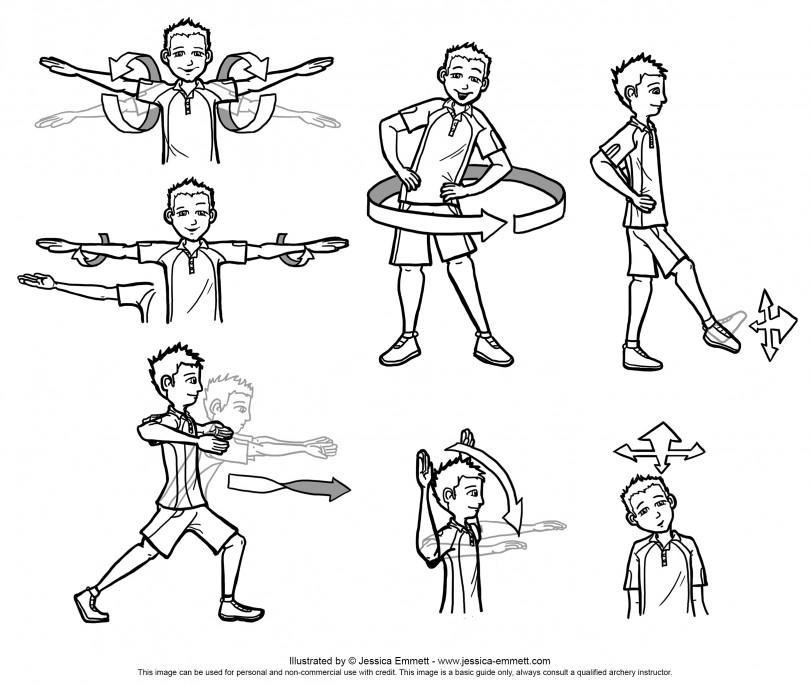
\includegraphics[width=1.0\textwidth]{./Figures/warmup.jpg}}
\end{figure}

\end{frame}

\begin{frame}
\frametitle{Warm up period}

\visible<1->{
\begin{figure}[ht]
\centerline{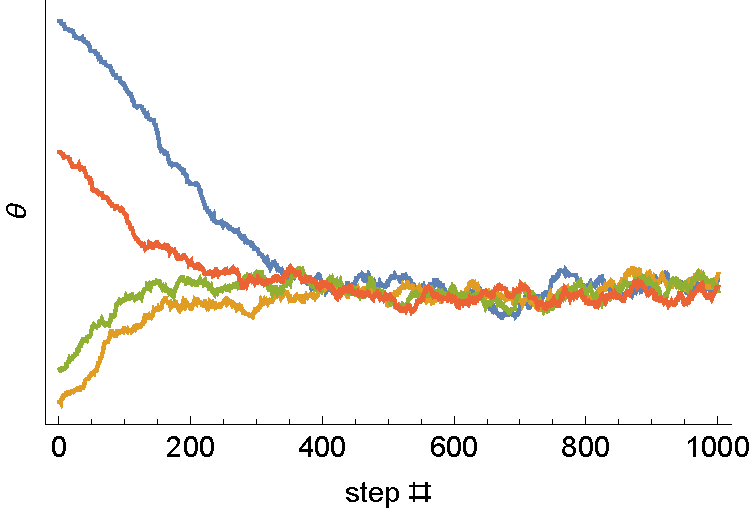
\includegraphics[width=1\textwidth]{./Figures/lec4_warmUp1.pdf}}
\end{figure}}

\end{frame}

\begin{frame}
\frametitle{Warm up period}

\visible<1->{
\begin{figure}[ht]
\centerline{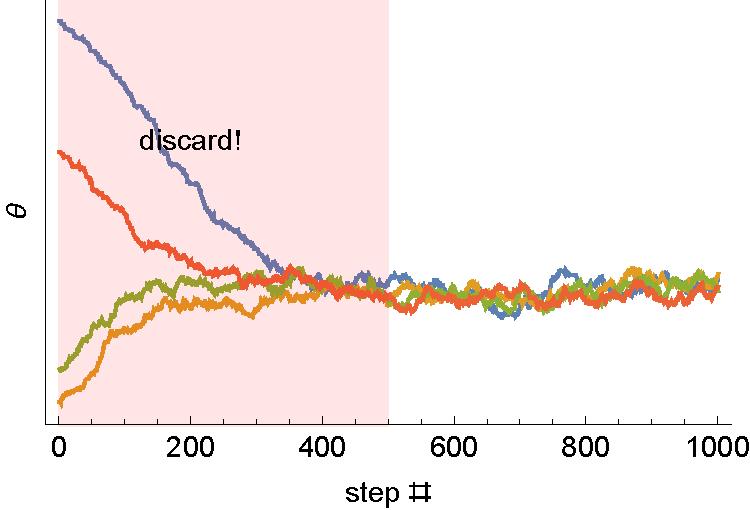
\includegraphics[width=1\textwidth]{./Figures/lec4_warmUp2.pdf}}
\end{figure}}

\end{frame}

\section{Adaptive covariance MCMC}
\frame{\tableofcontents[currentsection]}

\begin{frame}
	\frametitle{Inefficient exploration of the typical set by Random Walk Metropolis}
	
	\begin{figure}[t]
		\centerline{\animategraphics[width=0.7\textwidth,controls,buttonsize=1em,buttonfg=0.5]{2}{./Figures/lec5_MetropolisInefficient}{1}{50}}
	\end{figure}
	
\end{frame}

\begin{frame}
	\frametitle{Adaptive covariance MCMC: adjusting the proposal kernel to posterior geometry}
	
	\begin{itemize}
		\item The problem with RWM is that the proposals - being in random directions - are unlikely by chance to align with areas of high density.
		\item Adaptive covariance MCMC adjusts the proposal kernel dynamically to obtain a higher acceptance probability.
	\end{itemize}
	
\end{frame}

\begin{frame}
	\frametitle{Sketch of adaptive covariance algorithm(s)}
	
	Begin by generating $n$ samples using Random Walk Metropolis. Start with $\Sigma_0 = \text{identity matrix}$. Then,
	
	\begin{enumerate}
		\item Estimate sample mean: $\mu_t = \frac{1}{n}\sum_{i=1}^{t} \theta_i$.
		\item Estimate sample covariance matrix: $\Omega_t =  (\theta^{\{t\}}-\mu_t) (\theta^{\{t\}}-\mu_t)'$.
		\item Proposal kernel: $\Sigma_t = (1-a^t) \Sigma_{t-1} + a^t \Omega_t$.
	\end{enumerate}
	
	$\lim\limits_{t\rightarrow\infty} a^t = 0$ is key to ensuring convergence to posterior distribution.
	
\end{frame}

\begin{frame}
	\frametitle{Adaptive covariance MCMC: adjusting the proposal kernel to posterior geometry}
	
	\begin{figure}[t]
		\centerline{\animategraphics[width=0.7\textwidth,controls,buttonsize=1em,buttonfg=0.5]{2}{./Figures/adaptive_cartoon}{1}{6}}
	\end{figure}
	
\end{frame}

\begin{frame}
	\frametitle{Adaptive covariance MCMC: summary}
	
	\begin{itemize}
		\item RWM is inefficient due to random directionality of proposals.
		\item Adaptive covariance MCMC dynamically changes proposal kernel to match (global) posterior geometry leading to significant speed ups.
		\item ACMCMC can be used whenever RWM can be $\implies$ very general algorithm; particularly useful for ODE and PDE models, where gradients of solution (necessary for HMC) are expensive.
		\item ACMCMC and loads of other algorithms are available in PINTS: \url{https://github.com/pints-team/pints}.
		\item Problem: adapting to global geometry often leads to very poor local exploration.
	\end{itemize}
	
\end{frame}


\section{Ordinary differential equations}
\frame{\tableofcontents[currentsection]}

\begin{frame}
	\frametitle{Example: bacterial growth}
	\begin{itemize}
		\item<2-> We carry out experiments where we inoculate agar plates with bacteria at time 0.
		\item<3-> At pre-defined time intervals we count the number of bacteria on each plate, $N(t)$.
		\item<4-> Suppose we want to model bacterial population growth over time.
	\end{itemize}
	
	\onslide<1->
	\begin{figure}[ht]
		\centerline{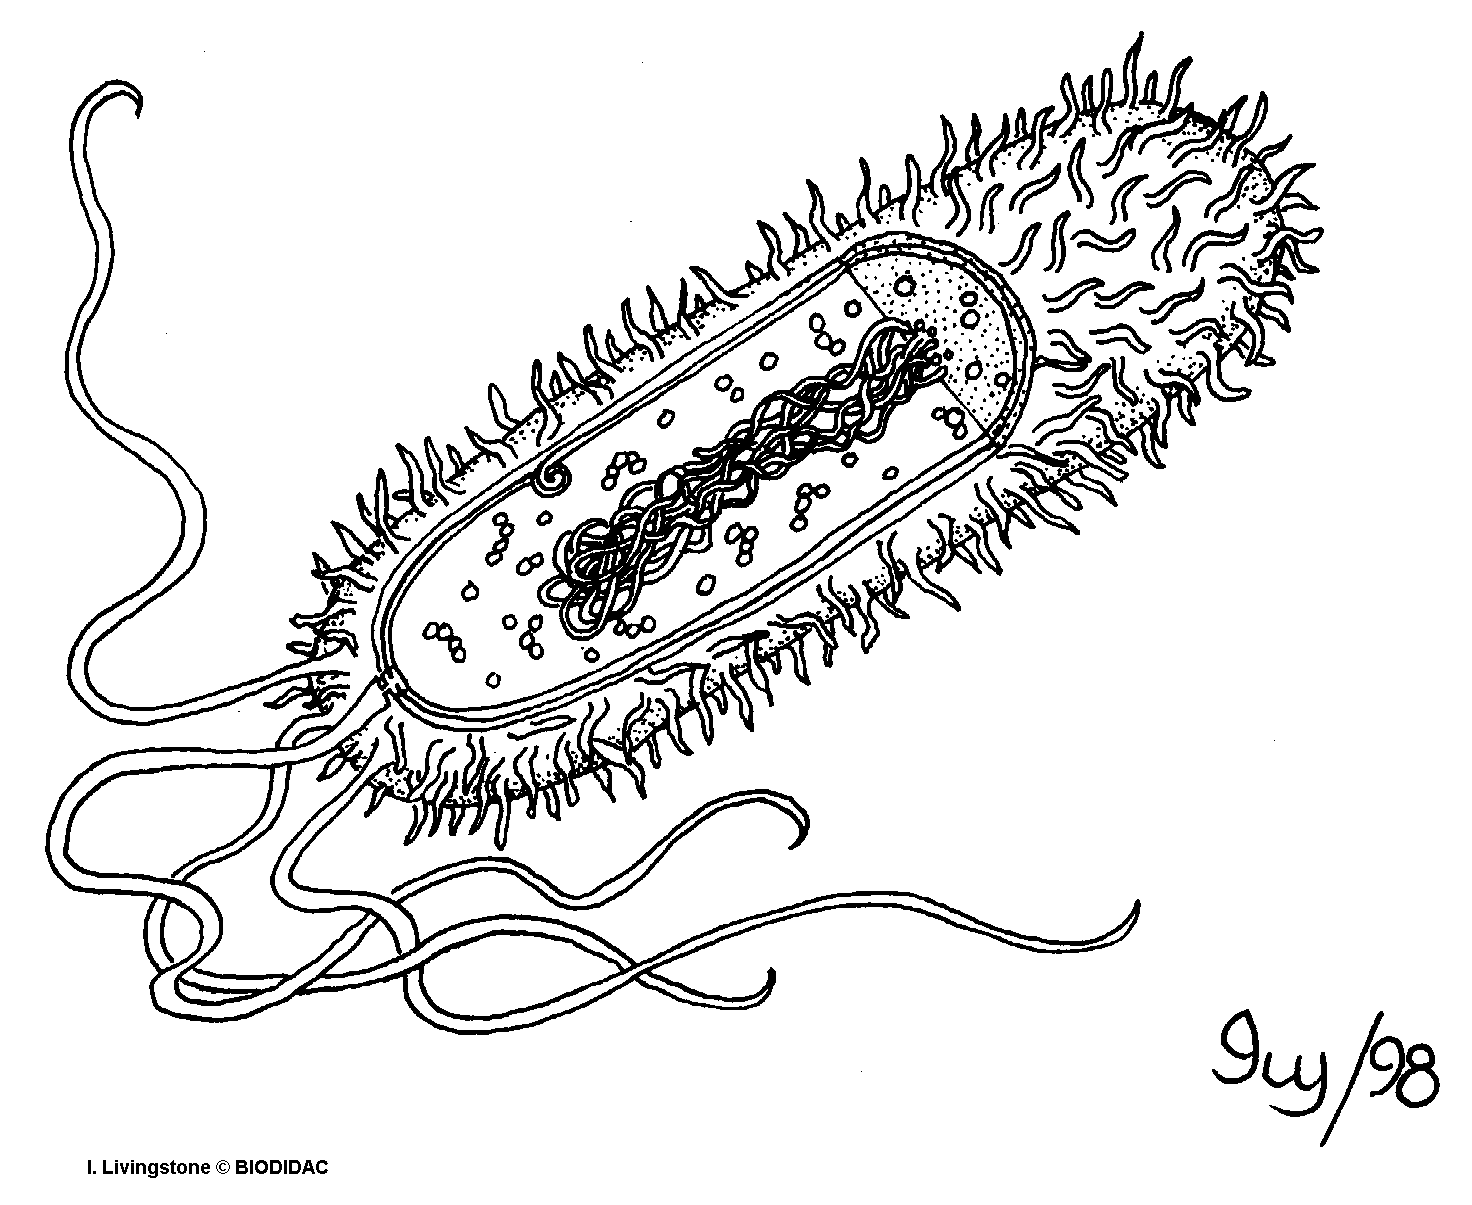
\includegraphics[width=1\textwidth]{./Figures/bacteria.png}}
	\end{figure}
	
\end{frame}

\begin{frame}
	\frametitle{Example: bacteria growth data}
	
	\begin{figure}[ht]
		\centerline{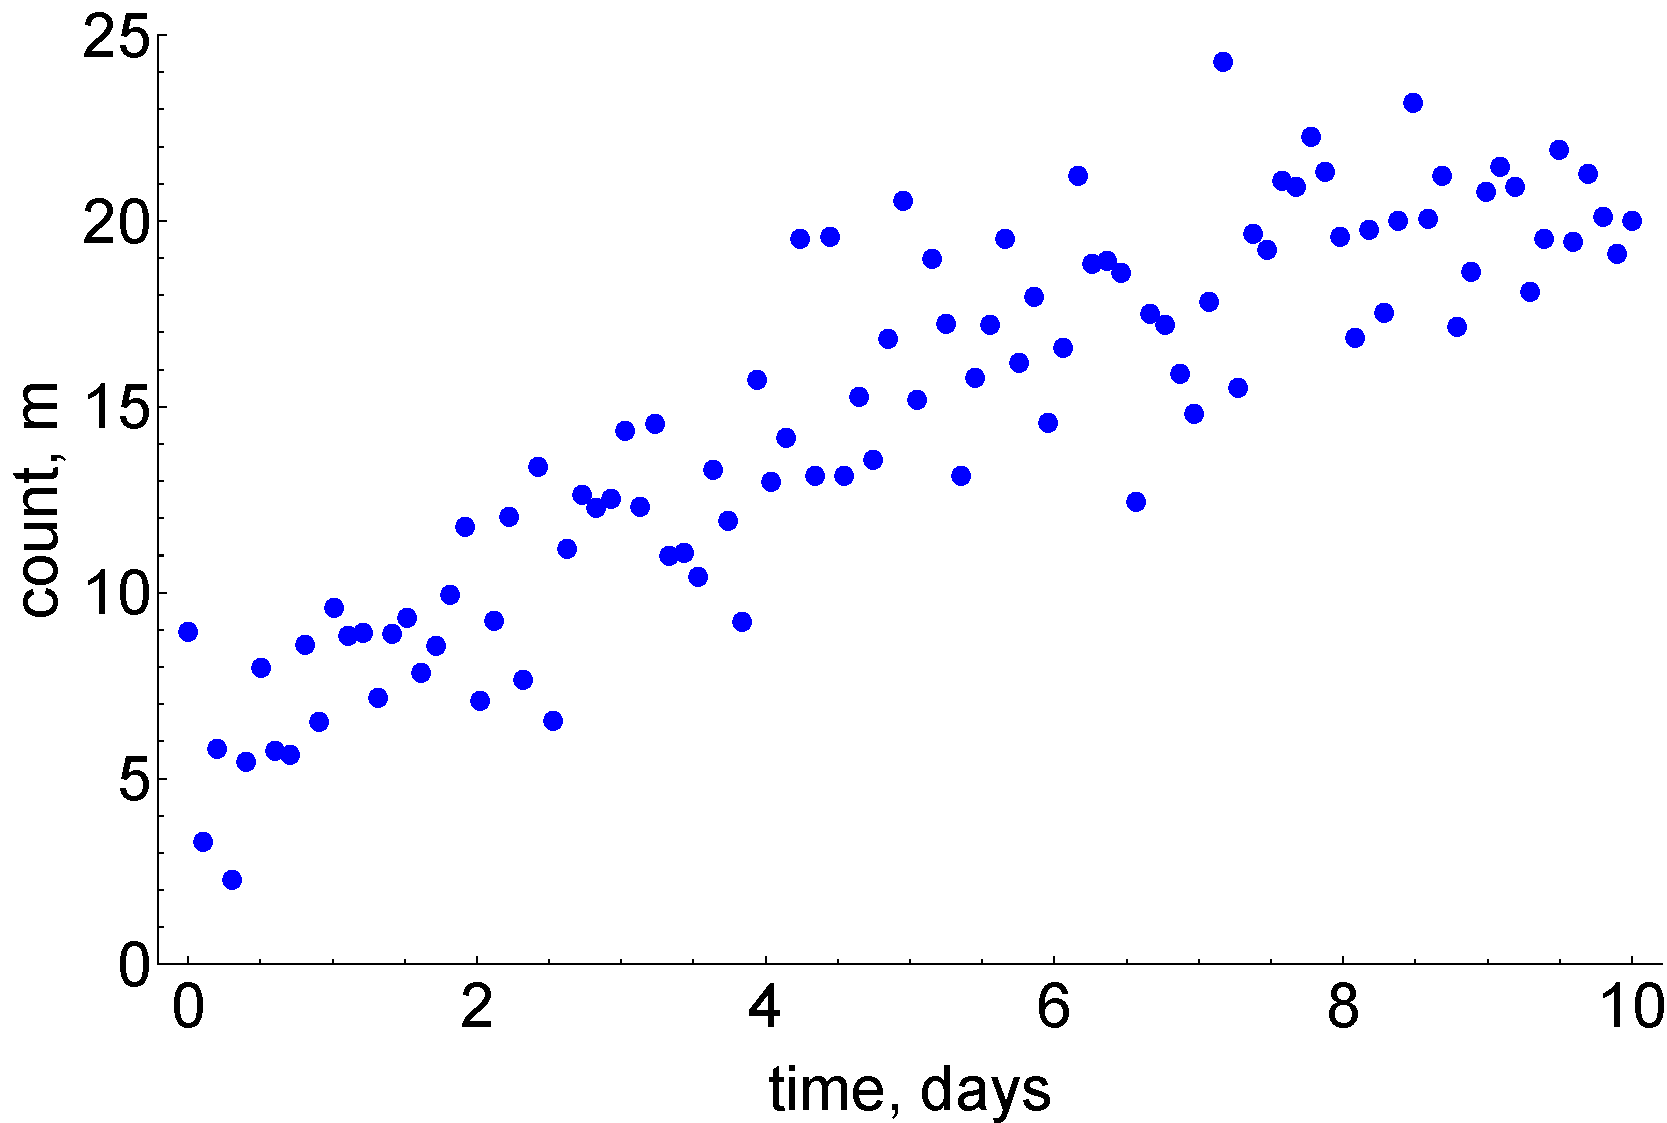
\includegraphics[width=1\textwidth]{./Figures/lec7_odeSingle.pdf}}
	\end{figure}
	
\end{frame}

\begin{frame}
	\frametitle{Example: bacterial growth model}
	\begin{itemize}
		\item<2-> Assume the following model for bacterial population growth:
	\end{itemize}
	
	\onslide<3->
	\begin{equation}
	\frac{\mathrm{d}N}{\mathrm{d}t} = \alpha N (1-\beta N)
	\end{equation}
	
	\onslide<4->
	where $\alpha>0$ is the rate of growth due to bacterial cell division, and $\beta>0$ measures the reduction in growth rate due to ``crowding''. 
	
	\onslide<5->
	\textbf{Question:} how should we infer the parameters of this model?
	
\end{frame}

\begin{frame}
	\frametitle{Example: bacterial growth model}
	\onslide<2->
	\textbf{Answer:} assume measurement error around true value:
	
	\onslide<3->
	\begin{equation}
	N^*(t) \sim \text{normal}(N(t), \sigma)
	\end{equation}
	
	\onslide<4->
	where
	\begin{itemize}
		\item<5-> $N^*(t)$ is the \textbf{measured} count of bacteria at time $t$.
		\item<6-> $N(t)$ is the solution to the ODE at time $t$ (true number of bacteria on plate).
		\item<7-> $\sigma>0$ measures the magnitude of the measurement error about the true value.
	\end{itemize}
	
	\onslide<8-> \textbf{Question:} how does this model work?
	
\end{frame}

\begin{frame}
	\frametitle{Example: bacterial growth model}
	Start with true number of bacterial cells, $N(t)$.
	
	\onslide<2->
	\begin{figure}[ht]
		\centerline{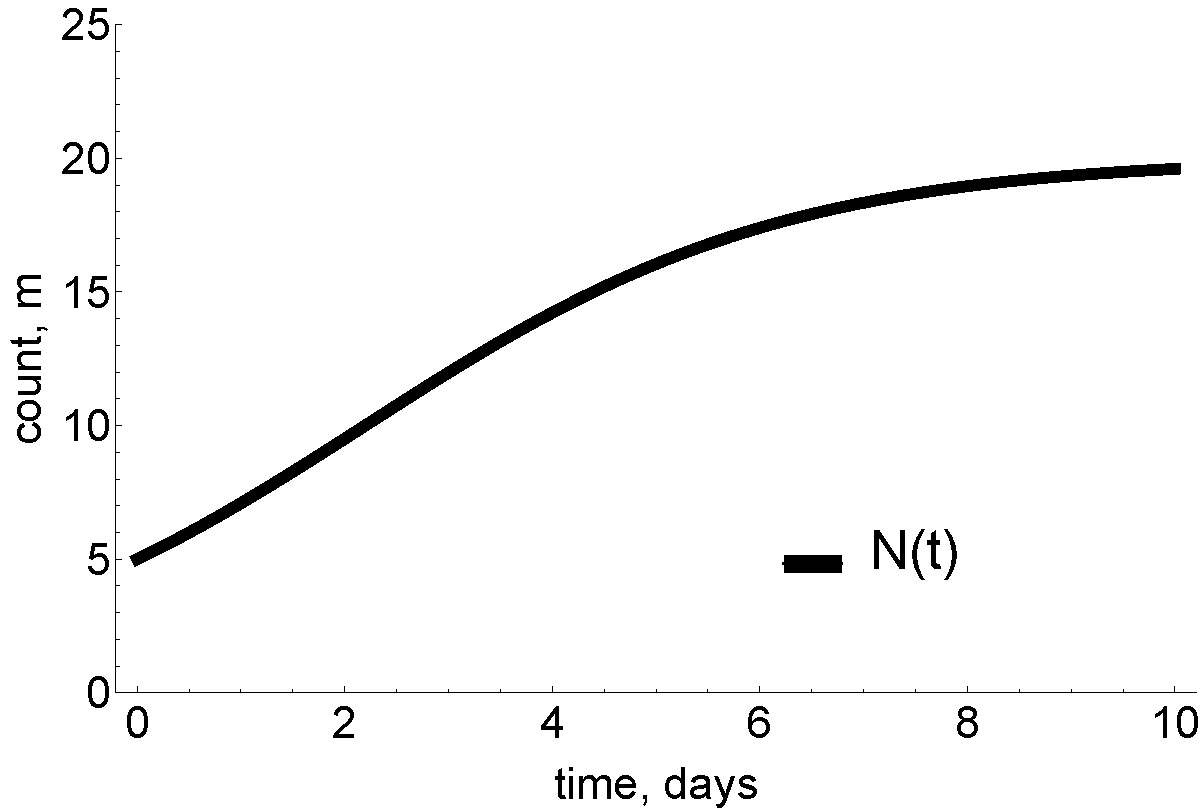
\includegraphics[width=1\textwidth]{./Figures/lec7_odeSingleBulding1.pdf}}
	\end{figure}
	
\end{frame}

\begin{frame}
	\frametitle{Example: bacterial growth model}
	Overlay sampling distribution representing measurement error.
	
	\begin{figure}[ht]
		\centerline{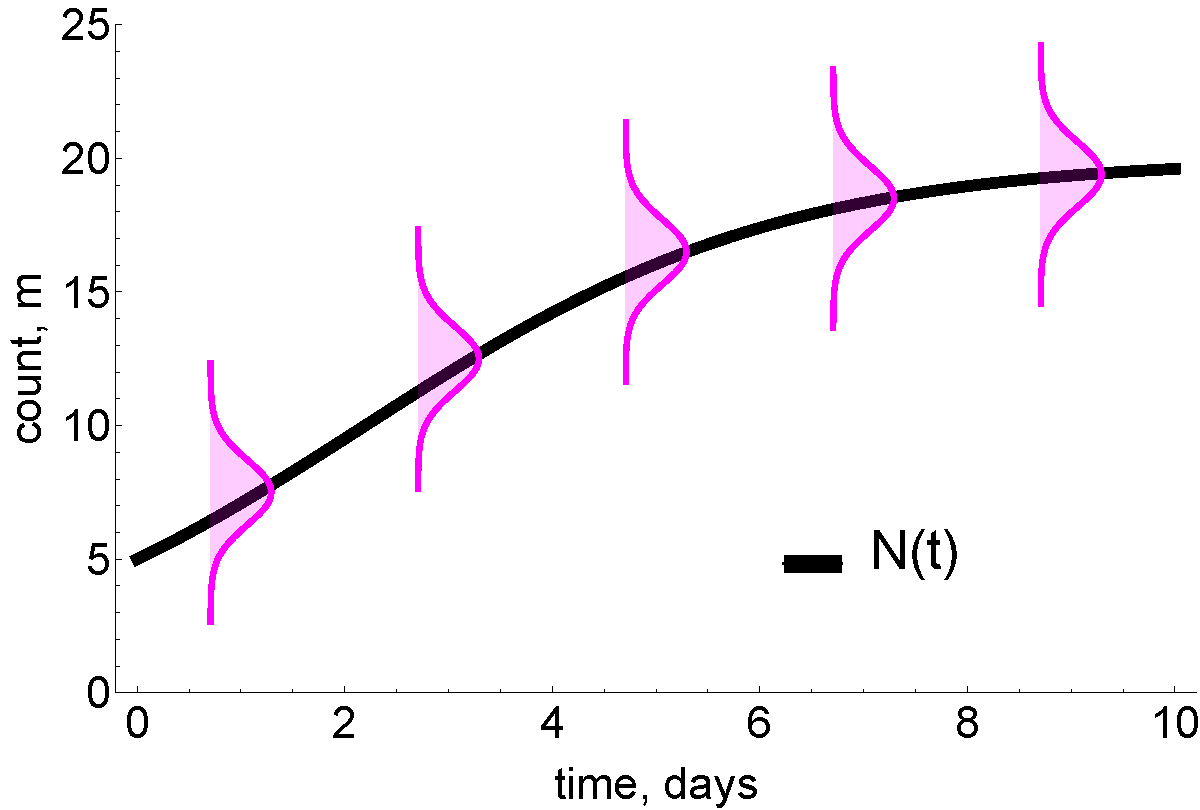
\includegraphics[width=1\textwidth]{./Figures/lec7_odeSingleBulding2.pdf}}
	\end{figure}
	
\end{frame}

\begin{frame}
	\frametitle{Example: bacterial growth model}
	And data generated from this process.
	
	\begin{figure}[ht]
		\centerline{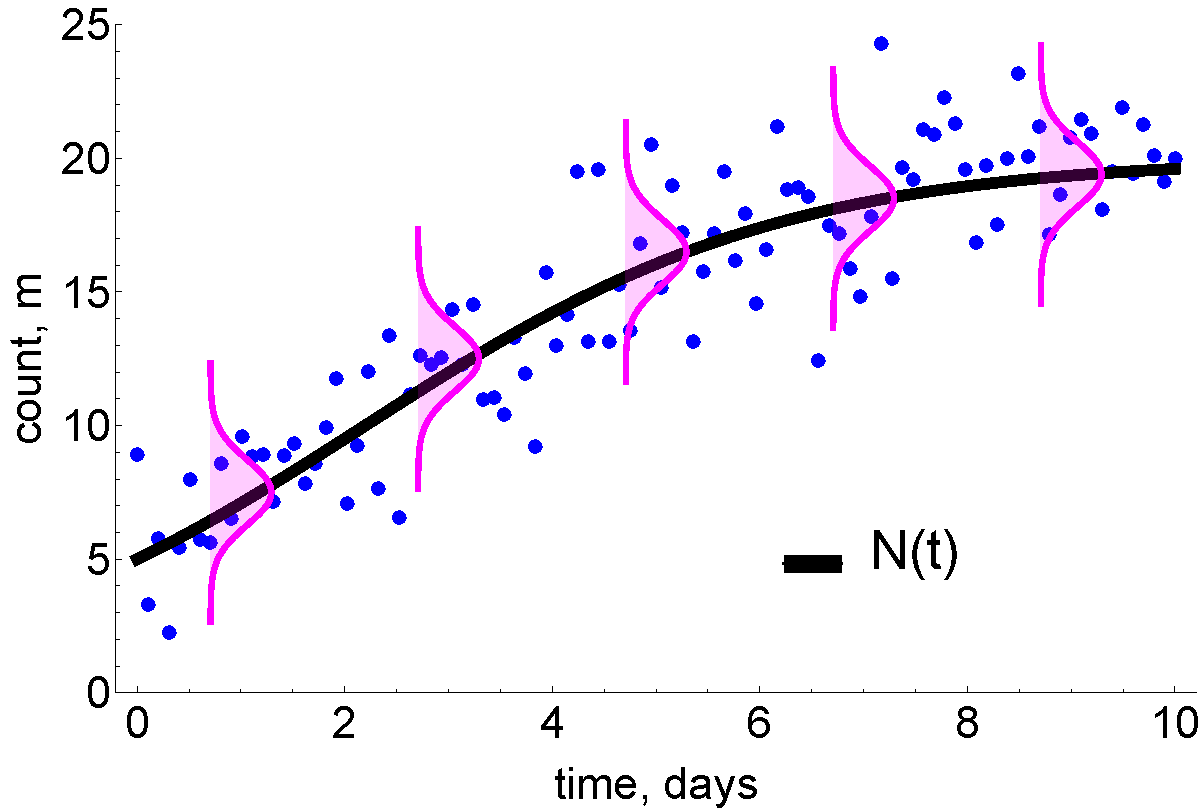
\includegraphics[width=1\textwidth]{./Figures/lec7_odeSingleBulding3.pdf}}
	\end{figure}
	
\end{frame}

\begin{frame}
	\frametitle{Example: bacteria growth model inference}
	\onslide<2-> Remember we are using a normal likelihood:
	
	\onslide<3->
	\begin{equation}
	N^*(t) \sim \text{normal}(N(t), \sigma)
	\end{equation}
	
	\onslide<4->
	$\implies$ likelihood for all observations:
	
	\onslide<5->
	\begin{equation}
	L(N(t),\sigma) = \prod_{t={t_1}}^{T} \frac{1}{\sqrt{2\pi\sigma^2}} exp\left[\frac{-(N^*(t) - N(t))^2}{2\sigma^2}\right]
	\end{equation}
	
	\onslide<6->
	\textbf{Question:} how do we calculate $N(t)$?
	
\end{frame}

\begin{frame}
	\frametitle{Example: bacteria growth model inference}
	
	\begin{equation}
	\frac{\mathrm{d}N}{\mathrm{d}t} = \alpha N (1-\beta N)
	\end{equation}
	
	\begin{itemize}
		\item<2-> In most ODE models, the mean $N(t)$ cannot be solved for exactly so we \textbf{can't write down a ``closed-form'' expression for the likelihood.}
		\item<3-> $\implies$ approximate answer using a numerical method.
		\item<4-> However any solution for $N(t)$ - exact or numerical - depends on the parameters of the ODE model. For our example:
		
		\onslide<5->
		
		\begin{equation}
		N(t) = f(t,\alpha,\beta)
		\end{equation}
		
	\end{itemize}
	
	\vspace{0.2cm}
	
	\onslide<6->
	\textbf{Question:} how do we do MCMC in this setting?
	
\end{frame}

\begin{frame}
	\frametitle{Example: bacteria growth model inference}
	
	\onslide<2-> For example, in Random Walk Metropolis:
	
	\begin{itemize}
		\item<3-> Start at random location in $(\alpha,\beta,\sigma)$ space.
		\item<4-> For t=1,...,T do:
		\begin{enumerate}
			\item<5-> Propose a new location $(\alpha',\beta',\sigma')$ using a jumping distribution.
			\item<6-> Numerically (or analytically) integrate ODE to solve for $N(t,\alpha',\beta')$.
			\item<7-> Calculate un-normalised posterior at proposed location $\implies$ calculate $r$.
			\item<8-> Based on $r$ move to new location or stay at original.
		\end{enumerate}
	\end{itemize}
	
	\onslide<9->
	$\implies$ at every step we must solve ODE for $N(t)$; can be computationally expensive!
	
\end{frame}

\begin{frame}
	\frametitle{Issues with inference for ODEs and PDEs}
	\begin{itemize}
		\item<2-> ODE models are very often non-identifiable $\implies$ need to reparameterise model.
		\item<3-> (Linked) ODE models can be slower to converge than simpler models $\implies$ need to run MCMC for longer before $\hat{R}<1.1$ achieved.
	\end{itemize}
	
	\onslide<4->
	$\implies$ important that we ``know'' our model well before we start to do inference explicitly.
	
	\onslide<5-> Worth putting energy into mathematical analysis before trying MCMC. 
	
\end{frame}


\begin{frame}
	\frametitle{Inference for ODEs: summary}
	\begin{itemize}
		\item<2-> ODE models are no harder to formulate than ``traditional'' problems.
		\item<3-> However for ODE models we cannot typically write down a ``closed-form'' expression for the likelihood.
		\item<4-> $\implies$ use integrator to numerically solve for mean for each set of parameters.
		\item<5-> Posteriors for ODE models are often of a more complex geometry than regular models and are often unidentified.
		\item<6-> Check out: \url{https://github.com/pints-team/pints} for ODE inference.
	\end{itemize}
	
\end{frame}

\end{document}
